\documentclass[12pt]{article}
\usepackage{fancyhdr} % for header
\usepackage{graphicx} % for figures
\usepackage{amsmath}  % for extended math markup
\usepackage{amssymb}  % "" (more math symbols)
\usepackage[bookmarks=false]{hyperref} % for URL embedding
\usepackage[noend]{algpseudocode} % for pseudocode
\usepackage[plain]{algorithm} % float environment for algorithms
\usepackage{subcaption}

\usepackage{geometry}
\geometry{a4paper, margin=1in}

\title{Project Deliverable 4: Final Project Writeup}
\author{Accelerating Molecular Dynamics on CUDA GPU}
\date{}

\begin{document}
\maketitle

\section*{Group Members}
% List all group members here:
\begin{itemize}
    \item Member 1: Charlie Li
    \item Member 2: Jack Yang
\end{itemize}

\section{Abstract}
% Provide a high-level overview of the project.
Molecular dynamics (MD) provides insight into the mechanisms of macromolecule folding and can guide the development of novel materials. Past MD research on linear monopolymers has found that chain length significantly influences folding behaviors, but current sequential algorithms require an unrealistic run time on a typical system of polymers with $N=1,000$ - $10,000$ particles. The bottleneck of an MD simulation is the pairwise force computation. Here, we parallelized force computations on CUDA GPUs with two approaches: exact computations and cutoff methods. Compared to the sequential version, the exact computation kernels achieved 30x - 100x speedup, while the cutoff methods demonstrated near-constant run times and up to 1000x speedup. Performance analysis reveals low occupancy as the main bottleneck at smaller $N$, with most kernels being compute bound at larger $N$. While the exact methods produce the desirable ensemble properties, the cutoff methods deviate significantly from expected behaviors even after energy corrections. Future work should be directed to fixing the physical flaws in the cutoff methods, as well as adapting the kernels to larger, non-linear systems and during the analysis stage.

\section{Introduction} \label{sec:intro}
% Provide background and significance of the project.
Molecular dynamics (MD) is a computational technique that simulates the movement of atoms across space and time in a molecular system. Providing reproducible trajectories of molecule motion with atom-level resolution, MD is an indispensable tool in fields like polymer chemistry and molecular biology to probe the mechanism of macromolecule folding.

Polymer chains demonstrate complex physical phenomena, notably temperature-induced phase transitions between globular and extended configurations. In space technology, linear monopolymers are widely used for thermal insulation and radiation shielding. However, the extreme temperatures in deep space causes polymers to fold and become brittle, which compromises their mechanical properties.

MD is well suited to exploring the effect of temperature on polymer folding. Under highly controlled simulation environments, variables like bond length and interaction strength can be tuned readily to optimize folding behavior of the monopolymer, which guides the development of cold-resistant materials. Past research with MD simulation has shown that polymer length significantly influences its phase transition behaviors. Increasing the length from $N=5$ to $80$ causes a notable decrease in normalized radius of gyration at a given temperature, indicating a tendency of longer chains to stay folded under the same conditions.

However, MD simulations are extremely time consuming. Furthermore, to optimize polymer behavior, an extensive parameter grid must be searched, with multiple rounds of MD run on each combination of parameters across different temperatures. To make this search computationally feasible, acceleration of the MD algorithm is much desired. The previous implementation of the sequential algorithm struggles with a system size of $N=100$, while the length of a typical industrial polymer chain ranges from 1,000 to 10,000. Therefore, significant (10x - 100x) speedup of the MD algorithm is required to perform accurate simulations on real-life systems and draw physically sound conclusions.

\section{Problem Statement}
% Describe the computational problem addressed.
The core computational problem is the calculation of non-bonded pairwise forces between a large system of $N$ particles over discrete time steps. In an MD simulation, every particle exerts a force on every other particle. In our specific model of a linear monopolymer, there are two classes of interactions formulated by the displacement vector $\vec{r}$ between two particles:
\begin{itemize}
    \item \textbf{Bonded Interactions} modeled by the harmonic potential:
    \[U_{bond}(r)=\frac{1}{2}k(r-r_0)^2\]
    \[\vec{F}_{bond}(\vec{r})=-k(|\vec{r}|-r_0)\frac{\vec{r}}{|\vec{r}|}\]
    where $r_0=1$ is the equilibrium bond length.
    \item \textbf{Non-bonded interactions} modeled by the Lennard-Jones potential, where $\epsilon$ is the energy well depth, and $\sigma$ is the distance at which the potential energy is $0$. There are two classes of non-bonded interactions.
    \begin{itemize}
        \item \textbf{Attraction} 
        \[ U_{attractive}(r)=4\epsilon_{attractive}\left[ \left(\frac{\epsilon}{r}\right)^{12} - \left(\frac{\epsilon}{r}\right)^{6} \right] \]
        \begin{equation*}
            \vec{F}_{attractive}(\vec{r})= 
                -\frac{24\epsilon_{attractive}}{|\vec{r}|}\left[\left(\frac{\sigma}{|\vec{r}|}\right)^6-2\left(\frac{\sigma}{|\vec{r}|}\right)^{12}\right]\frac{\vec{r}}{|\vec{r}|}
        \end{equation*}
        \item \textbf{Repulsion}
        \begin{equation*}
            U_{attractive}(r)=\begin{cases}
                4\epsilon_{attractive}\left[ \left(\frac{\epsilon}{r}\right)^{12} - \left(\frac{\epsilon}{r}\right)^{6} \right] & r<2^{1/6}\sigma\\
                0 & r\ge 2^{1/6}\sigma
            \end{cases}
        \end{equation*}
        \begin{equation*}
            \vec{F}_{repulsive}(\vec{r})=\begin{cases}
                 -\frac{24\epsilon_{repulsive}}{|\vec{r}|}\left[\left(\frac{\sigma}{|\vec{r}|}\right)^6-2\left(\frac{\sigma}{|\vec{r}|}\right)^{12}\right]\frac{\vec{r}}{|\vec{r}|} & |\vec{r}|<2^{1/6}\sigma \\
                 0 & |\vec{r}|\ge 2^{1/6}\sigma
            \end{cases}
        \end{equation*}
    \end{itemize}
\end{itemize}

In the simplest model, a pair of particles exerts a single class of force on each other, where $i$ and $j$ are the indices of the particles on the polymer chain:
\begin{equation*}
    \vec{F}_{i,j} = \begin{cases}
        \vec{F}_{bond}(\vec{r_j}-\vec{r_i}) & |j-i|=1 \\
        \vec{F}_{repulsive}(\vec{r_j}-\vec{r_i}) & |j-i|=2 \\
        \vec{F}_{attractive}(\vec{r_j}-\vec{r_i}) & |j-i|\ge 3
    \end{cases}
\end{equation*}

The net force on each particle is the sum of all $N-1$ forces from other particles, which naively requires $O(N^2)$ computations.

MD simulates the trajectory of atom movements over time by repeatedly computing the forces, deriving acceleration by Newton’s second law, and integrating over an extremely small timestep on the magnitude of femtoseconds. Since most other steps scale linearly with the number of atoms, the step of force computation is rate-limiting. To see notable motion of the system, a large number ($10^6-10^{12}$) of such time steps needs to be performed. Coupled with the large number of particles in a typical system, calculating the $O(N^2)$ forces for each step on a CPU quickly becomes computationally intractable.

Since the computation of forces on one atom does not affect that on another atom in a given timestep where their positions do not change, this force computation is highly parallelizable. The goal of this project is to map this massively data-parallel workload onto the GPU to achieve a significant speedup.

\section{Approach}
% Detail the methods and techniques used.
\subsection{Exact Computations}
In this approach, each and every pair of forces are computed exactly. Naively, we can map a thread to each particle and calculate the forces from all the other particles. That is the approach of the segmented traversal kernel. However, Newton's third law states that the action and the reaction between a pair of particles have the same magnitude. Therefore, it is a waste of computing power to re-compute that same force on the other particle, which is an expensive operation given the extensive exponentiation in force computation. We implemented two kernels to take advantage of this equality and minimize computation: the explicit force matrix and the implicit force matrix.

\subsection{Label-Cutoff Method}
\begin{figure}[h]
    \centering
    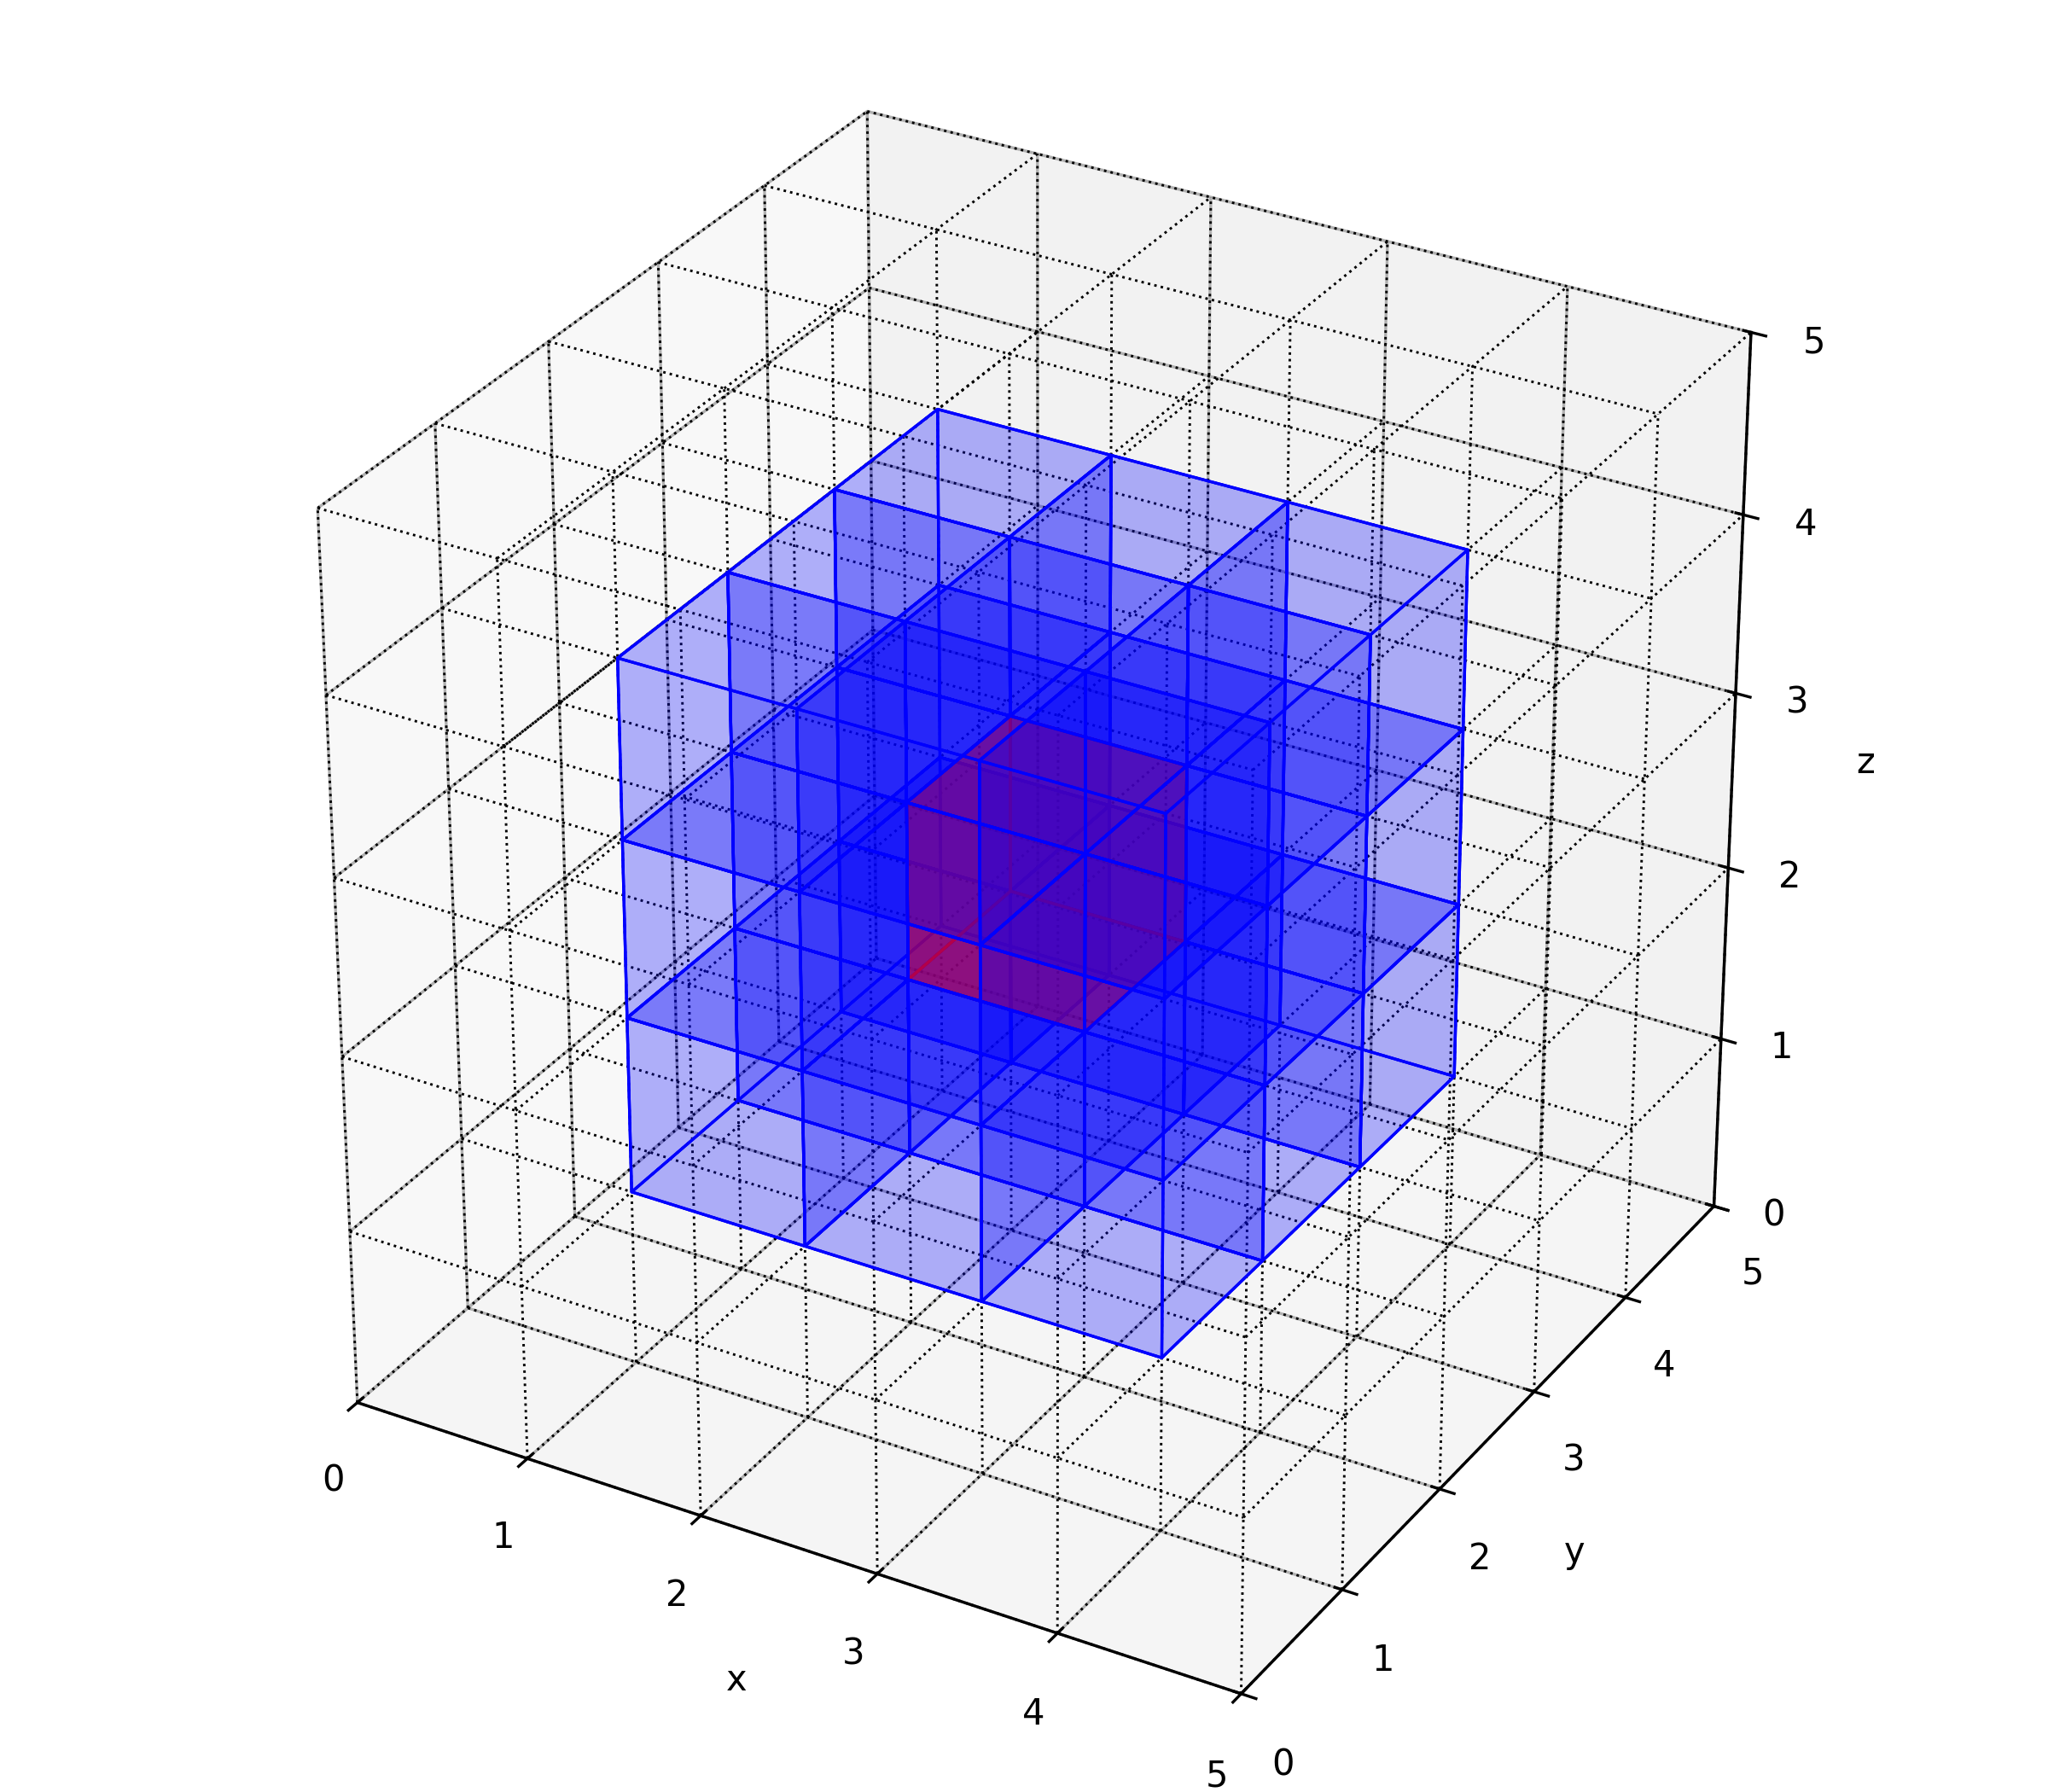
\includegraphics[width=0.5\linewidth]{cutoff_illustration.png}
    \caption{Illustration of Label/Cutoff Algorithm}
    \label{fig:cut_illus}
\end{figure}
Since the Lennard-Jones interaction scales with $r^6$, it is negligible when distance is large. The overall idea of the cutoff-distance method is to divide the simulation box into many small cells, where each cell may contain multiple atoms or may be empty. Then for one atom inside a home cell, we do not compare it with all other atoms in the system. Instead, we only check atoms inside its own cell (red cell) and the 26 surrounding cells (blue cells), so in total 27 cells shown in Figure~\ref{fig:cut_illus}. After that, even for atoms inside those candidate cells, we still only compute the interaction if the actual pair distance is within the cutoff. In our current implementation, the cutoff is $r_c=2.5\sigma$, which is a conventional value in MD simulations. This assumption lets us ignore many pairwise computations without changing the result too much. Because of this, the force evaluation is much cheaper than the original all-pairs method.

Truncation of Lennard-Jones forces leads to a discontinuity of the potential energy at the cutoff as well as systematic errors in potential energy.

To smooth out the attractive Lennard-Jones potential energy at the cutoff, the following shift is applied:
\begin{equation*}
    U_{attractive}^{shifted}(r)=\begin{cases}
        U_{attractive}(r)-U_{attractive}(r_c) & r\le r_c\\
        0 & r>r_c
    \end{cases}
\end{equation*}

The standard Long-Range Corrections (LRC) are applied to correct for the long-range interactions, assuming a uniform density when $r>r_c$, where $r_c$ is the cutoff distance:
\[ U_{tail} = \frac{8}{3}\pi\rho\epsilon\sigma^3\left[ \frac{1}{3}\left(\frac{\sigma}{r_c}\right)^9 - \left(\frac{\sigma}{r_c}\right)^3 \right] \]

\section{Implementation}
% Include details of the implementation, including optimization steps taken.

\subsection{Exact Computations}
\subsubsection{Compare: Sequential Code}
The sequential algorithm is implemented with a doubly nested loop, which calculates forces for each unique pair once and accumulates them to the global forces array. The pseudocode is shown in algorithm \ref{algo:sequentialExact}. There are in total $\frac{N(N-1)}{2}$ force calculations performed in this algorithm, and its time complexity is $O(N^2)$, where $N$ is the number of particles.
\begin{algorithm}
\caption{Sequential Exact Computations} \label{algo:sequentialExact}
\begin{algorithmic}[1]
\State{fill(forces, 0)}
\For{$i=0$ to $n-2$}
    \For{$j=i+1$ to $n-1$}
        \State{displacement = minimum\_image\_between(positions[i], positions[j])}
        \State{distance = norm(displacement)}
        \State{f = compute\_force\_between(i, j, distance)*displacement/distance}
        \State{forces[i] += f}
        \State{forces[j] -= f}
    \EndFor
\EndFor
\end{algorithmic}
\end{algorithm}

Three different kernels are implemented that compute the forces on each atom exactly.

\subsubsection{Segmented Traversal}
The segmented traversal algorithm is a straightforward GPU implementation of force computation. In this algorithm, each thread is mapped to one atom, and it loops through all the other atoms and adds the forces into a local register variable. Finally, it stores the net force on that atom into the global forces array. The pseudocode is shown in algorithm \ref{algo:segmentedTraversal}

\begin{algorithm}
\caption{Segmented Traversal} \label{algo:segmentedTraversal}
\begin{algorithmic}[1]
\State $idx \gets \text{Global Thread ID}$
\State $tid \gets \text{Local Thread ID}$
\State $N \gets \text{Total number of particles}$
\State $\mathbf{p}_{recv} \gets \mathbf{positions}[idx]$ \Comment{Register array of receiver positions}
\State $\mathbf{F}_{local} \gets \mathbf{0}$ \Comment{Register force accumulator}
\State $\mathbf{p}_{src} \gets \text{Shared Array of size } SEGMENT$ \Comment{Source positions tile}

\For{$start = 0$ \textbf{to} $N - 1$ \textbf{step} $SEGMENT$}

    \Comment{Cooperative tile loading into shared memory}
    \State $\mathbf{p}_{src}[tid] \gets \mathbf{positions}[start + tid]$
    \State \Call{SyncThreads}{}
    
    \Comment{Pairwise force calculation for current tile}
    \For{$i = 0$ \textbf{to} $SEGMENT-1$}
        
        \State $\mathbf{F}_{local} \gets \mathbf{F}_{local} + \mathbf{F}_{idx,start+i}$
    \EndFor
    \State \Call{SyncThreads}{}
\EndFor

\State $\mathbf{forces}[idx] \gets \mathbf{F}_{local}$
\end{algorithmic}
\end{algorithm}

\subsubsection{Explicit Force Matrix}
Although the segmented traversal kernel is clean and achieves impressive speedup, it wastes half of the computation work, since according to Newton’s Third Law, the magnitude of the forces are the same between a pair of atoms. The explicit force matrix kernel attempts to reduce unnecessary computations by paying the cost of more global memory operations. We envision a $N\times N$ force matrix, with each entry recording the force from the row atom (source) to the column atom (receiver). We only need to calculate the upper triangular part of this matrix, and the lower triangular entries can be filled by taking the negative of the entry at its transposed position. The pseudocode for filling the force matrix is shown in algorithm \ref{algo:explicitMatrix}, and that for the parallel reduction is shown in algorithm \ref{algo:matrixReduction}

\begin{algorithm}
\caption{Filling the Explicit Force Matrix} \label{algo:explicitMatrix}
\begin{algorithmic}[1]
\State $idx \gets \text{Global Thread ID}$
\State $N \gets \text{Total number of particles}$
\State $n \gets N - 1$ \Comment{Exclude diagonal entries}

\Comment{Map 1D thread ID to 2D upper triangular indices (row, col)}
\State $row \gets \left\lceil n - 0.5 - \frac{\sqrt{(2n+1)^2 - 8(idx+1)}}{2} \right\rceil$
\State $col \gets idx + row - \frac{(2n-row+1)row}{2} + 1$

\State $\mathbf{p}_{src} \gets \mathbf{positions}[row]$ \Comment{Register array of source position}
\State $\mathbf{p}_{recv} \gets \mathbf{positions}[col]$ \Comment{Register array of receiver position}

\Comment{Pairwise force calculation and global memory write}
\State $\mathbf{forces\_mat}[idx] \gets \mathbf{F}_{row,col}$
\end{algorithmic}
\end{algorithm}

\begin{algorithm}
\caption{Explicit Matrix Reduction} \label{algo:matrixReduction}
\begin{algorithmic}[1]
\State $col \gets \text{Global Block ID}$ \Comment{Target particle index}
\State $tid \gets \text{Local Thread ID}$
\State $N \gets \text{Total number of particles}$
\State $n \gets N - 1$
\State $CF \gets \text{Coarsening factor}$
\State $\mathbf{F}_{local} \gets \mathbf{0}$ \Comment{Register force accumulator}
\State $\mathbf{S} \gets \text{Shared Array of size } BLOCK\_DIM$ \Comment{Shared memory for reduction}

\Comment{Thread-coarsened accumulation handling matrix symmetry}
\For{$idx = tid \times CF$ \textbf{to} $(tid + 1) \times CF - 1$}
    \If{$idx = col$}
        \State \textbf{continue}
    \EndIf
    
    \State $r \gets idx, \quad c \gets col, \quad sign \gets 1$
    \If{$r > c$}
        \State \Call{Swap}{$r, c$}
        \State $sign \gets -1$
    \EndIf
    
    \State $mat\_idx \gets \frac{(2n - r + 1)r}{2} + c - 1 - r$ \Comment{1D index mapping}
    \State $\mathbf{F}_{local} \gets \mathbf{F}_{local} + sign \cdot \mathbf{forces\_mat}[mat\_idx]$
\EndFor

\State $\mathbf{S}[tid] \gets \mathbf{F}_{local}$
\State \Call{SyncThreads}{}

\Comment{Parallel tree reduction in shared memory}
\State $step \gets BLOCK\_DIM / 2$
\While{$step > 0$}
    \If{$tid < step$}
        \State $\mathbf{S}[tid] \gets \mathbf{S}[tid] + \mathbf{S}[tid + step]$
    \EndIf
    \State $step \gets step / 2$
    \State \Call{SyncThreads}{}
\EndWhile

\Comment{Write reduced net force to global memory}
\If{$tid = 0$}
    \State $\mathbf{forces}[col] \gets \mathbf{S}[0]$
\EndIf
\end{algorithmic}
\end{algorithm}

\subsubsection{Implicit Force Matrix}
The explicit force matrix requires a large chunk of global memory and leads to highly irregular global memory accesses to the collapsed storage array that cannot be coalesced. We implemented the implicit force matrix algorithm, which uses atomic operations to accumulate local sums directly into the global forces array without the need to maintain the intermediate results. In this algorithm, the force matrix is implicit, i.e. it is a conceptual and organizational framework instead of a real data structure. The pseudocode is shown in algorithm \ref{algo:implicitMatrix}

\begin{algorithm}
\caption{Implicit Force Matrix} \label{algo:implicitMatrix}
\begin{algorithmic}[1]
\State $bid \gets \text{Global Block ID}$
\State $tid \gets \text{Local Thread ID}$
\State $b_{row}, b_{col} \gets \text{Map } bid \text{ to 2D upper triangular tile indices}$
\State $recv\_idx \gets b_{col} \times TILE\_DIM + tid$
\State $src\_offset \gets b_{row} \times TILE\_DIM$

\State $\mathbf{p}_{src} \gets \text{Shared Array of size } TILE\_DIM$ \Comment{Source positions tile}
\State $\mathbf{F}_{col} \gets \mathbf{0}$ \Comment{Register force accumulator for receiver}

\Comment{Cooperative tile loading into shared memory}
\State $\mathbf{p}_{src}[tid] \gets \mathbf{positions}[src\_offset + tid]$
\State \Call{SyncThreads}{}

\If{$b_{row} == b_{col}$} \Comment{Diagonal tile handling}
    \State $\mathbf{p}_{recv} \gets \mathbf{p}_{src}[tid]$ \Comment{Receiver position is already in shared memory}
    
    \For{$i = 1$ \textbf{to} $sweep-1$} \Comment{Start at 1 to skip self-interaction}
        \State $src\_idx \gets (i + tid) \pmod{sweep}$ \Comment{Cyclic shift avoids bank conflicts}
        \State $\mathbf{F}_{col} \gets \mathbf{F}_{col} + \mathbf{F}_{recv\_idx, \ src\_offset + src\_idx}$
    \EndFor
    \State \Call{AtomicAdd}{$\mathbf{forces}[recv\_idx], \mathbf{F}_{col}$}

\Else \Comment{Non-diagonal tile handling}
    \State $\mathbf{F}_{row} \gets \text{Shared Array of size } TILE\_DIM$ \Comment{Force accumulator for sources}
    \State $\mathbf{F}_{row}[tid] \gets \mathbf{0}$
    \State \Call{SyncThreads}{}

    \State $\mathbf{p}_{recv} \gets \mathbf{positions}[recv\_idx]$ \Comment{Load receiver from global memory}
    
    \For{$i = 0$ \textbf{to} $sweep-1$}
        \State $src\_idx \gets (i + tid) \pmod{sweep}$
        \State $\mathbf{f} \gets \mathbf{F}_{recv\_idx, \ src\_offset + src\_idx}$
        
        \State $\mathbf{F}_{col} \gets \mathbf{F}_{col} + \mathbf{f}$
        \State \Call{AtomicAdd}{$\mathbf{F}_{row}[src\_idx], -\mathbf{f}$} \Comment{Newton's Third Law}
    \EndFor
    
    \State \Call{AtomicAdd}{$\mathbf{forces}[recv\_idx], \mathbf{F}_{col}$}
    \State \Call{SyncThreads}{}
    
    \Comment{Cooperative writeback of source forces to global memory}
    \State \Call{AtomicAdd}{$\mathbf{forces}[src\_offset + tid], \mathbf{F}_{row}[tid]$}
\EndIf
\end{algorithmic}
\end{algorithm}

\subsection{Label-Cutoff Method}
\subsubsection{Sequential Cutoff}
The sequential version of this method is exactly the same as the Algorithm~\ref{algo:sequentialExact} except that before the computation it will decide whether to skip this force or not the force applied by this atom shown in Algorithm~\ref{algo:sequentialCutoff}. This skip will save a lot of computation without significantly influence the final progressing of the molecule chain.

\begin{algorithm}
\caption{Sequential Cutoff Computations} \label{algo:sequentialCutoff}
\begin{algorithmic}[1]
\State{fill(forces, 0)}
\For{$i=0$ to $n-2$}
    \For{$j=i+1$ to $n-1$}
        \State{displacement = minimum\_image\_between(positions[i], positions[j])}
        \State{distance = norm(displacement)}
        \If {distance $>$ cutoff} \Comment{*Change here}
            \State Skip
        \EndIf
        \State{f = compute\_force\_between(i, j, distance)*displacement/distance}
        \State{forces[i] += f}
        \State{forces[j] -= f}
    \EndFor
\EndFor
\end{algorithmic}
\end{algorithm}

\subsubsection{Label/Cutoff Method}
In our design, the whole method on GPU can be divided into three phases: Label, Sort, and Compute.

The first phase is the Label phase illustrated in Algorithm\ref{algo:atomLabel}. In this phase, we assign one cell label to each atom based on its current position. Suppose the box is divided into dim cells in each direction, and each cell has width \texttt{cell\_size}. Then for one atom, we compute \texttt{cell\_x}, \texttt{cell\_y}, and \texttt{cell\_z} by dividing its coordinate by cell\_size and taking the integer part. Since positions are already inside the box, the cell index in each direction is nonnegative. Then the 3D cell index is converted into one 1D label by \texttt{cell\_x + cell\_y*dim + cell\_z*dim*dim}. We store these labels in a temporary array of size n, the number of atoms. This phase is very suitable for parallelism because each atom is processed independently, and there is no communication or race condition between threads. Also, the memory access pattern for reading each position and writing to each label are both coalesced which improves the performance and minimizes the divergence between warps.

\begin{algorithm}[h]
\caption{Atom Label Kernel} \label{algo:atomLabel}
\begin{algorithmic}[1]

\State Compute global thread index: \texttt{idx}
\If{\texttt{idx} is outside the valid atom range}
    \State Return
\EndIf

\State 
\State $x \gets \texttt{positions}[0,\texttt{idx}]$
\State $y \gets \texttt{positions}[1,\texttt{idx}]$
\State $z \gets \texttt{positions}[2,\texttt{idx}]$

\State 
\State $\texttt{cell\_x} \gets \lfloor x / \texttt{cell\_size} \rfloor$
\State $\texttt{cell\_y} \gets \lfloor y / \texttt{cell\_size} \rfloor$
\State $\texttt{cell\_z} \gets \lfloor z / \texttt{cell\_size} \rfloor$

\State 
\State $\texttt{cell\_x} \gets \texttt{cell\_x} \bmod \texttt{dim}$
\State $\texttt{cell\_y} \gets \texttt{cell\_y} \bmod \texttt{dim}$
\State $\texttt{cell\_z} \gets \texttt{cell\_z} \bmod \texttt{dim}$

\State 
\State $\texttt{label} \gets \texttt{cell\_x} + \texttt{cell\_y} \times \texttt{dim} + \texttt{cell\_z} \times \texttt{dim}^2$

\State 
\State $\texttt{labels[idx]} \gets \texttt{label}$

\end{algorithmic}
\end{algorithm}

The second phase is the Sort phase shown in Algorithm~\ref{neighbor_kernel}. In this phase, we sort atoms according to their cell labels, so atoms that belong to the same cell become consecutive in memory. After sorting, we reorder the position array in the same way, so the new position array is grouped by cell. Then we count how many atoms belong to each label by a histogram operation, and after that we do a prefix sum on this count array. This gives an array called \texttt{cell\_start}. The meaning of \texttt{cell\_start[c]} is the starting index of cell \texttt{c} in the sorted position array, and \texttt{cell\_start[c+1]} is the ending index. Therefore, all atoms inside cell \texttt{c} are exactly in the range from \texttt{cell\_start[c]} to \texttt{cell\_start[c+1]-1}. This makes neighbor-cell lookup very efficient, because once a neighboring cell id is known, we can directly jump to the corresponding range in the sorted array. One issue in this phase is that after sorting, the atom order is no longer the original chain order from the initial position array. Because of this, we also store another array called \texttt{org\_idx}, which records the original index of each atom before sorting. This is useful in our case because the force model depends not only on distance but also on the separation along the chain, for example distinguishing bonded, near-bonded, and non-bonded interactions. If the original order were not needed, then this method would be even more favorable, because after one timestep the positions are already partially grouped in space, which may reduce the sorting work in the next iteration. In our implementation, this whole phase is done by CuPy functions such as argsort, bincount, and cumsum. These operations are already highly optimized, so it is not necessary to manually write extra GPU kernels for them.

\begin{algorithm}[h]
\caption{Neighbor Retrieving Array Building} \label{algo:neighbor_kernel}
\begin{algorithmic}[1]
\State Sorting Atoms by Label to Quickly Find Neighbors
\State $\texttt{order} \gets \texttt{argsort}(\texttt{labels})$
\State $\texttt{labels\_sorted} \gets \texttt{labels}[\texttt{order}]$
\State $\texttt{positions} \gets \texttt{positions}[:, \texttt{order}]$
\State $\texttt{org\_idx} \gets \texttt{order}$
\State $\texttt{counts} \gets \texttt{bincount}(\texttt{labels\_sorted})$
\State $\texttt{cell\_start}[0] \gets 0$
\State $\texttt{cell\_start}[1:] \gets \texttt{cumsum}(\texttt{counts})$

\end{algorithmic}
\end{algorithm}

The last phase is the Compute phase illustrated in Algorithm~\ref{algo:force_compute}. In this phase, each atom is mapped to exactly one thread, and that thread computes the total net force acting on this atom. This design avoids race conditions, because each thread only writes to one force entry. The kernel first finds the home cell of the current atom, then loops over the 27 neighboring cells including the home cell. For each neighboring cell, it gets the corresponding atom range from \texttt{cell\_start}, then iterates through all atoms in that range. For each candidate atom pair, it computes the minimum-image displacement, then the pair distance, and if the distance is smaller than the cutoff, it evaluates the force and adds it to the local force accumulator. At the end, the thread writes the final x, y, and z force components back to global memory according to the index stored in \texttt{org\_idx}.
The sequential version follows almost the same logic as the parallel version. It still has the same three phases: labeling atoms, sorting by cell, building \texttt{cell\_start}, and then searching only over neighboring cells. The main difference is that all these operations are done in sequential loops instead of parallel GPU kernels or CuPy primitives. Therefore, the sequential version is mainly used as a reference implementation to verify correctness and compare runtime.

\begin{algorithm}
\caption{Cutoff Force Computation with Compact Cell List}\label{algo:force_compute}
\begin{algorithmic}[1]

\State Compute global atom index $i$
\If{$i$ is outside the valid atom range}
    \State Return
\EndIf

\State Read atom $i$ position and original index $i_o$
\State Compute the cell coordinates $(c_x, c_y, c_z)$ for atom $i$

\State Initialize total force:
\State \hspace{1em} $\mathbf{F}_i \gets (0,0,0)$

\For{each neighboring cell around $(c_x,c_y,c_z)$}
    \State Convert the 3D neighbor cell coordinate to a 1D label

    \State Use \texttt{cell\_start} to get the atom range of this neighbor cell

    \For{each atom $j$ in this neighbor cell}
        \If{$j=i$}
            \State Continue
        \EndIf

        \
        \State Compute displacement between atom $i$ and atom $j$
        \State Compute distance $r_{ij}$

        \If{$r_{ij}$ is too small or $r_{ij}$ is larger than the cutoff radius}
            \State Continue
        \EndIf

        \State Use the original indices $i_o$ and $j_o$ to determine bonded separation
        \State Compute pairwise force magnitude
        \State Accumulate force contribution to $\mathbf{F}_i$
    \EndFor
\EndFor

\State Write the final force back to the original atom index $i_o$

\end{algorithmic}
\end{algorithm}

\section{Optimizations Applied}

\textbf{Common Optimization: Memory Coalescing} A typical MD simulation is performed in three dimensional space, meaning that we need to store three parameters for each variable. To allow for memory coalescing for the GPU kernels, we structured the global positions, forces and velocities arrays in the layered format (with shape $3\times N$). Since neighboring threads in a warp access neighboring entries for the same dimensions in one instruction, the layered format allows coalesced read and write for each dimension. We implemented all GPU algorithms based on this data structure.

\subsection{Exact Computations}

\subsubsection{Segmented Traversal}
\textbf{Optimization: Shared Memory Tiling} Since every atom needs access to the positions of every other atom, there are lots of memory reuse opportunities. We optimized this algorithm by having threads in one block cooperate to load segments of the positions array into shared memory and calculate forces using the loaded positions.

\subsubsection{Explicit Force Matrix}
In a naive implementation, we could launch a kernel to fill this matrix, and then perform standard parallel reduction to sum the forces. However, we will need at least a memory size of $N^2 \text{ entries}\times 3 \frac{\text{dimension}}{\text{entry}} \times 8 \frac{\text{bytes}}{\text{dimension}}=24 N^2 \text{ bytes}$.

\textbf{Optimization: Collapsing the upper-triangular matrix} We do not necessarily need the lower triangular part of the force matrix, since it can be filled by taking the negative transposed upper triangular matrix. Therefore, we only need to store the upper triangular part of the matrix, which can be collapsed into a 1-dimensional array to space storage. With this method, we reduce the number of entries from $N^2$ to $\frac{N(N-1)}{2}$, and total storage is reduced to $12N(N-1)$.

\begin{figure}[htbp]
    \centering
    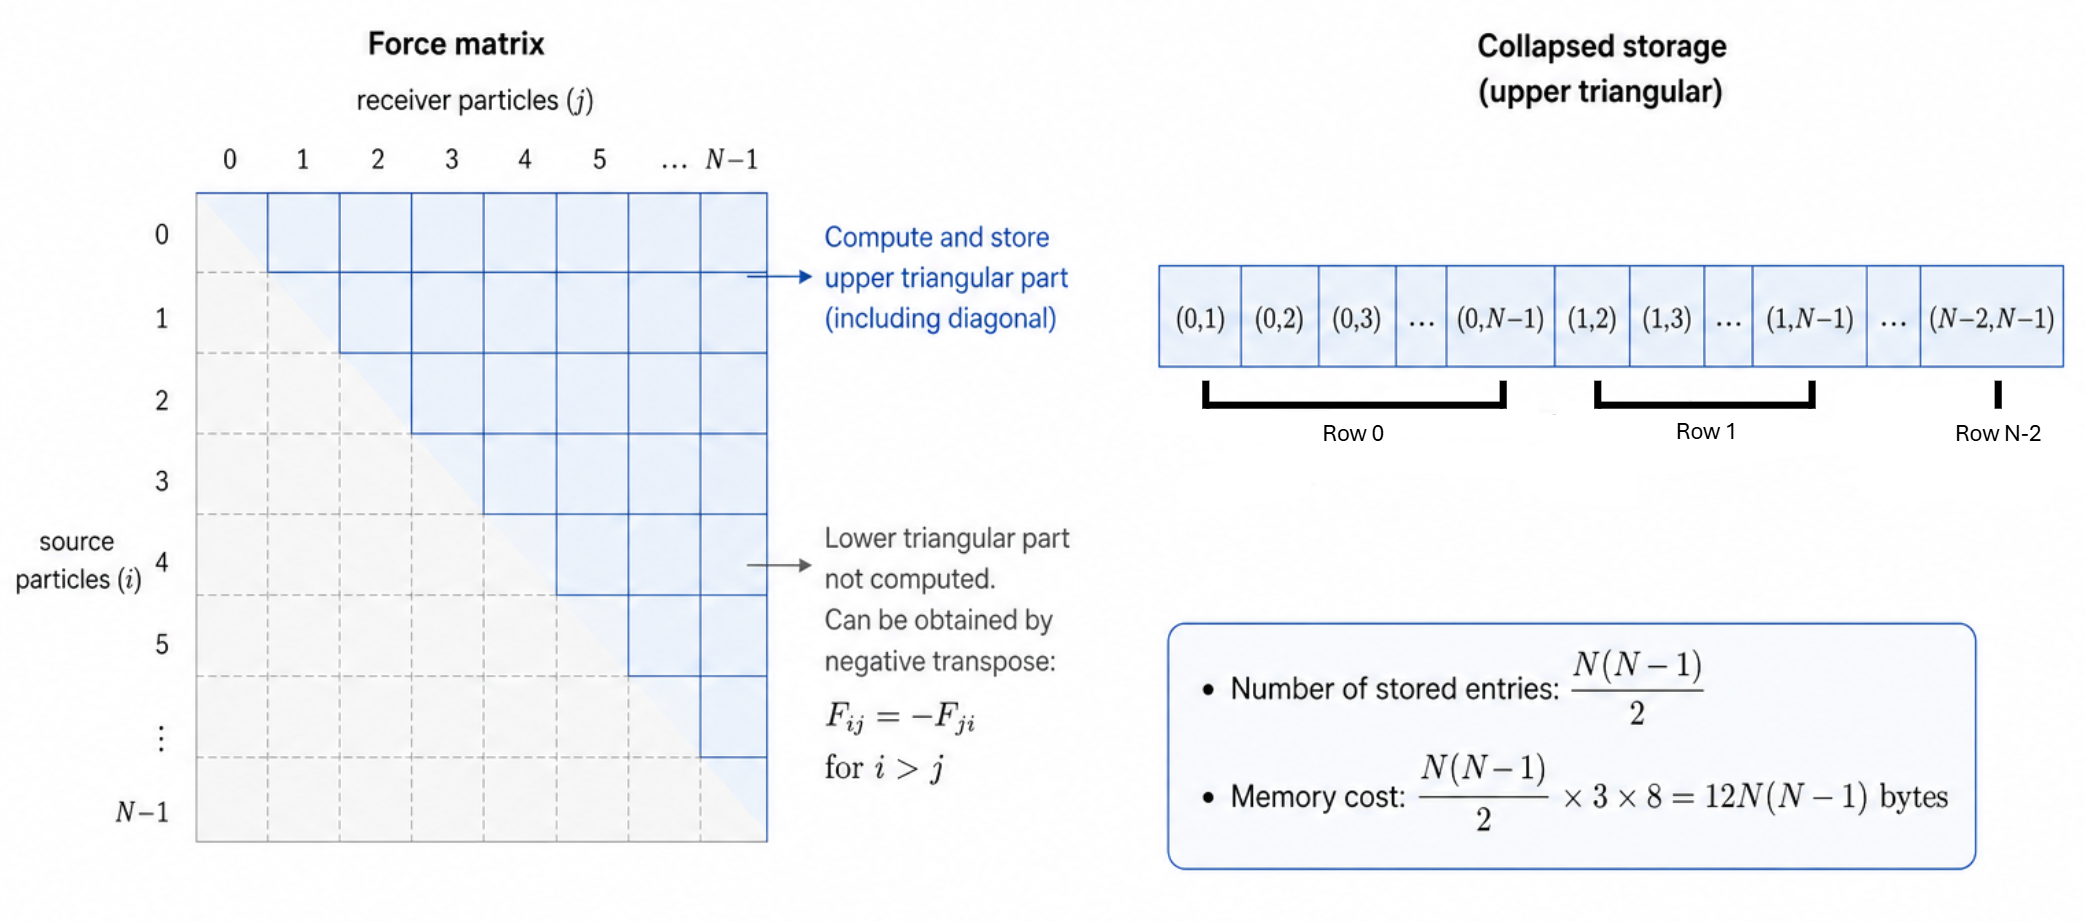
\includegraphics[width=0.8\linewidth, height=0.8\textheight, keepaspectratio]{explicit_matrix_illus.png}
    \caption{Illustration showing the collapsing of the force matrix. Image adopted from GPT Image 2.}
    \label{fig:explicit_matrix}
\end{figure}

To map coordinates $(r, c)$ in the upper triangular force matrix to the 1-dimensional index $b$ in the collapsed storage array: $b = \frac{(2N-r+1)r}{2} +c-r$

To map the 1-dimensional index $b$ to coordinates in the upper-triangular force matrix:
\begin{itemize}
    \item $r = \lceil n - 0.5 - \frac{\sqrt{(2N+1)^2-8(b+1)}}{2} \rceil $
    \item $c = b+r-\frac{(2N-r+1)r}{2}$ 
\end{itemize}

\textbf{Optimization: Parallel reduction with thread coarsening}
We adapted the standard parallel reduction algorithm to the collapsed storage format. One block of threads is launched on each column of the force matrix to perform parallel reduction and obtain the net force on each particle, with $N$ blocks in one kernel launch. Each thread is coarsened by a factor of $\lceil \frac{N}{BLOCK\_DIM}\rceil$, sequentially sums the neighboring entries according to the coarsening factor, and stores the sum into shared memory. The standard reduction tree is then performed on the shared memory array.

The only difference between our method and the standard parallel reduction is during the sequential sum stage (figure \ref{reduction}). Each thread first traverse the force matrix from top to bottom until they hit the diagonal, after which they traverse from left to right and use the negative of the forces to accumulate into shared memory.

\begin{figure}[htbp]
    \centering
    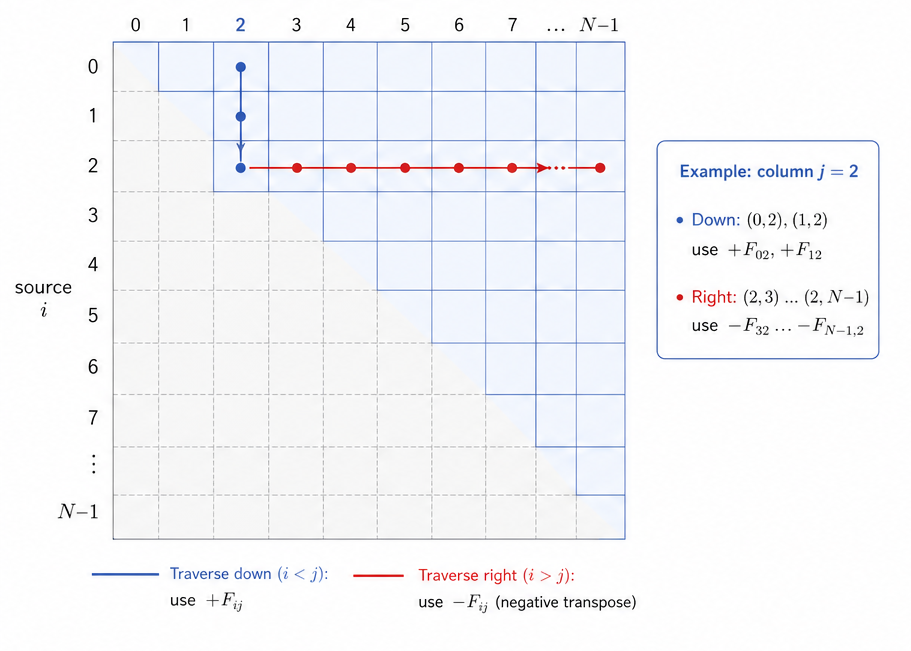
\includegraphics[width=0.8\linewidth, height=0.8\textheight, keepaspectratio]{parallel_reduction.png}
    \caption{Illustration showing the traversal of the force matrix made by one block during the sequential sum stage of parallel reduction. Image adopted from GPT Image 2.}
    \label{fig:reduction}
\end{figure}

\subsubsection{Implicit Force Matrix}
\textbf{Optimization: Shared memory tiling} We break the matrix into tiles and map blocks to tiles. Each block has t threads and maps to a tile of $t\times t$ atoms in the matrix. Each thread traverses the tile from top to bottom and computes the forces on one column (receiver) atom. The positions of the source (row) atoms are loaded into shared memory and re-used by all $t$ threads in the same block.

\textbf{Optimization: Privatization} To reduce global memory contentions, we accumulate the forces in registers or shared memory before adding them back to the global forces array. Since each thread loops through a column, it could keep a register accumulator for forces on the column atom. On the other hand, different threads need to access the accumulators for the row atoms. Therefore, the accumulators for the row atoms are stored in shared memory. In each iteration, a thread adds the force into its register accumulator variable, as well as the negative of that force into the corresponding position in shared memory.

\textbf{Optimization: Juxtaposition to reduce shared memory contention}
Although shared memory is much faster than global memory, contention still leads to costs in run time. In a naive implementation where all threads loop through the same rows, they all attempt to write to the same position in shared memory simultaneously. To minimize shared memory contention, we juxtapose the source atom indices processed by each thread in each iteration (figure \ref{fig:juxtapose}. In the $i^{th}$ iteration, thread $k$ will process the force of atom $(i+k)\bmod t$ on atom $k$. When $t<32$, there will be no shared memory contention, since threads in each warp operate on different positions in shared memory.

\begin{figure}[htbp]
    \centering
    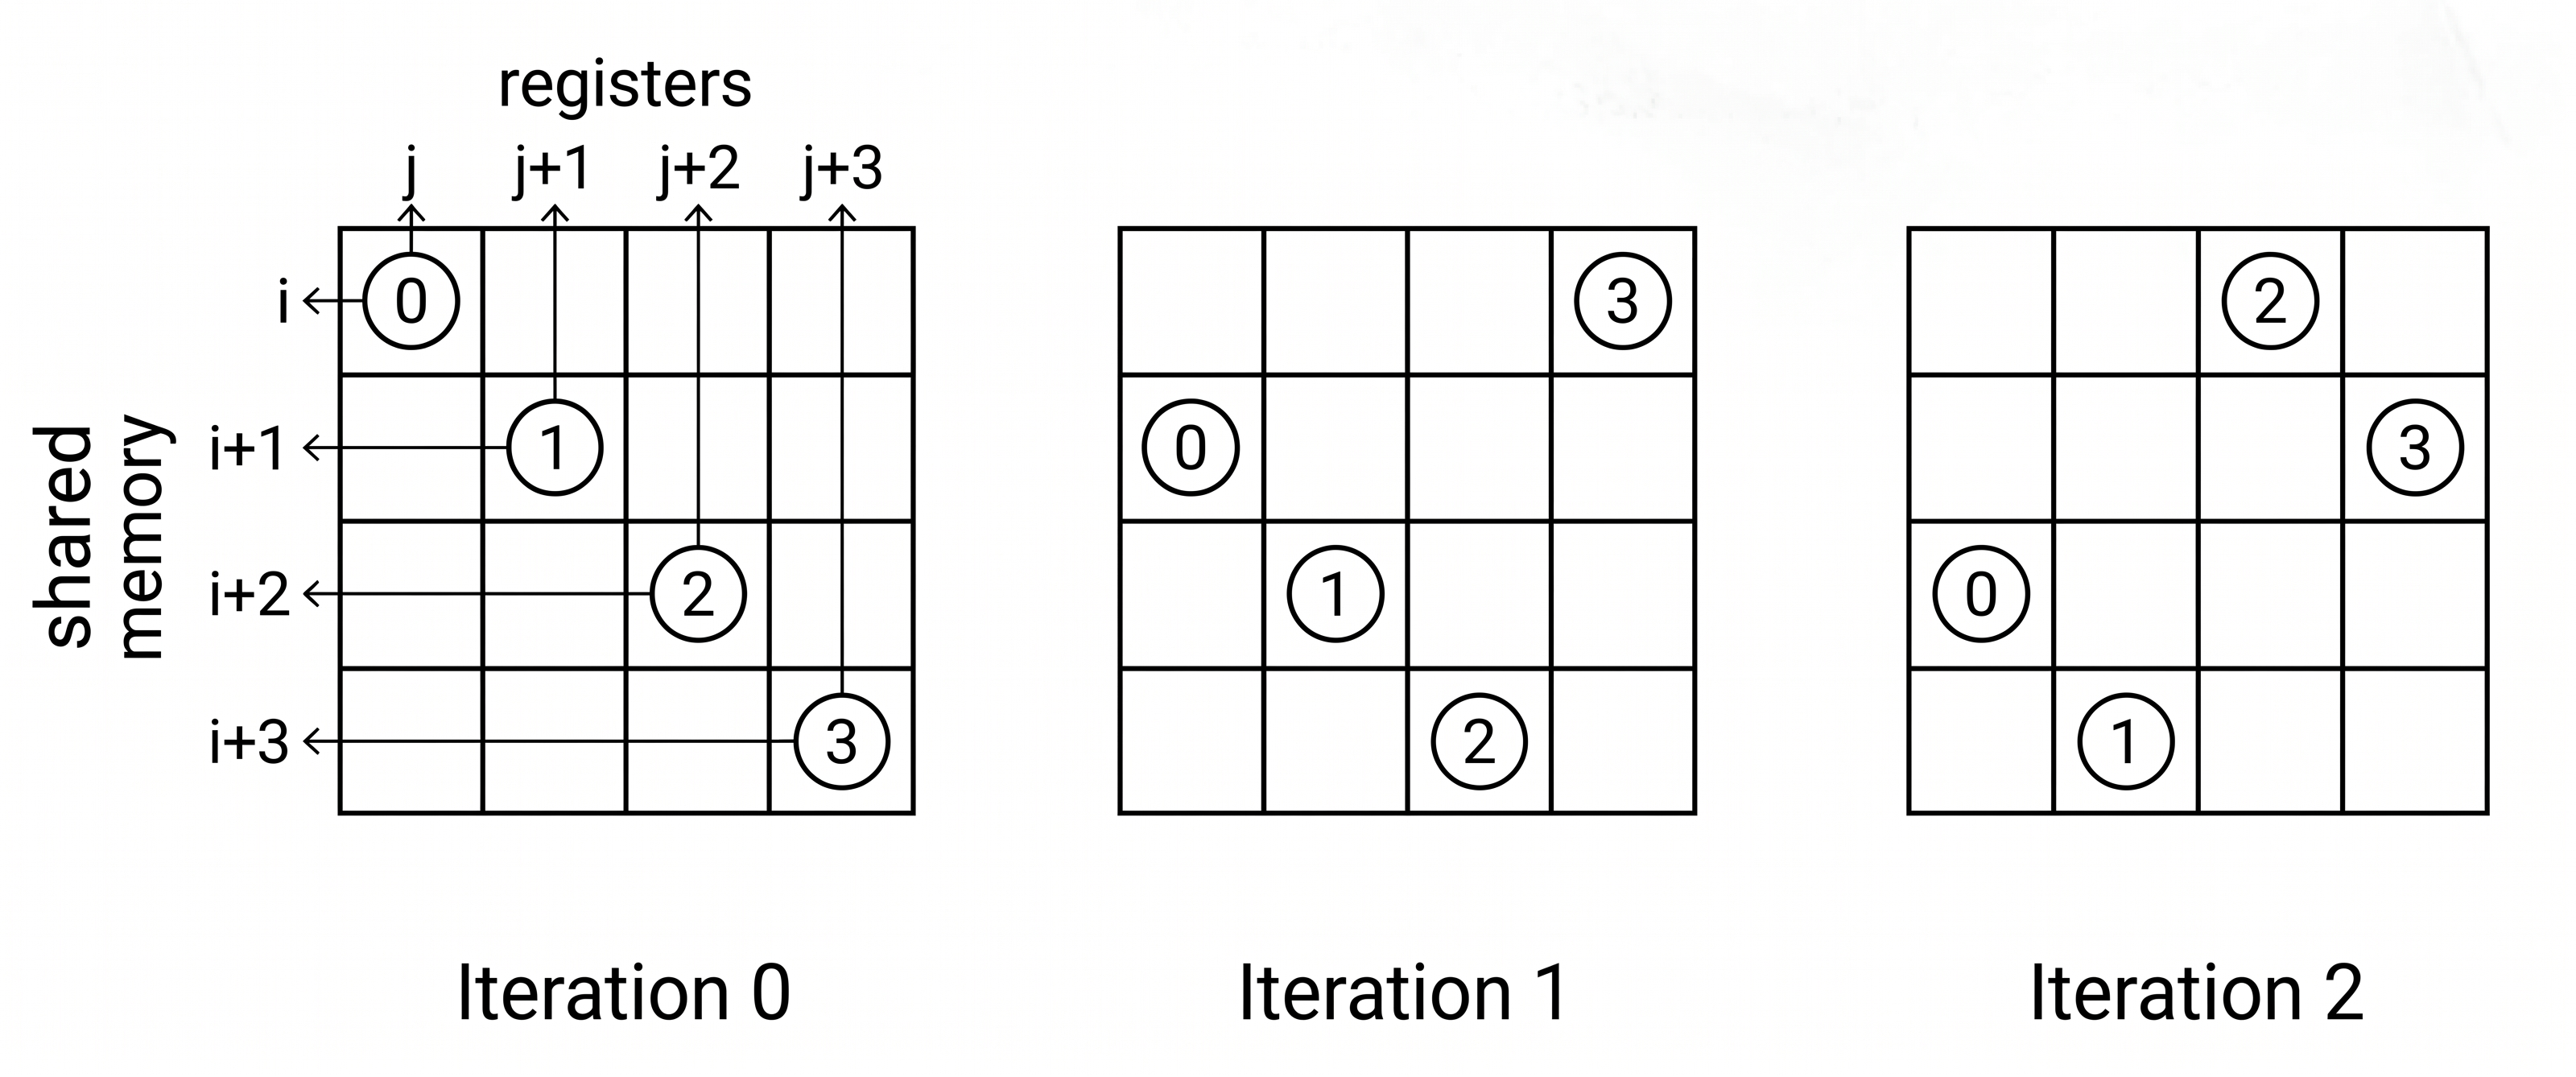
\includegraphics[width=0.8\linewidth, height=0.8\textheight, keepaspectratio]{implicit_matrix_juxtapose.png}
    \caption{Illustration of the juxtaposed traversal of one tile in the implicit force matrix. Image generated by Nano Banana.}
    \label{fig:juxtapose}
\end{figure}

\subsection{Label/Cutoff Optimization}

\subsubsection{Optimization 1: Sorted Position Recovery}

In this first optimization, we noticed that there is a repeated process in the second stage of each iteration. In the original implementation, the atom positions are sorted according to their cell labels. Two additional device arrays, \texttt{sorted\_positions} and \texttt{org\_idx}, are then used to store the sorted positions and the mapping back to the original atom order. This mapping is necessary because the force results must eventually be written back to the correct atoms in the original global arrays.

Instead of recovering the original position order after every iteration, we propose keeping the global \texttt{positions} array in sorted order. In this case, only the mapping array \texttt{org\_idx} needs to be updated each iteration. Since atoms usually move only a small distance during one timestep, their cell labels are expected to change only slightly. Therefore, the label array may remain partially sorted between iterations.

This optimization has two possible benefits. First, sorting partially sorted labels may be faster than sorting a fully unsorted array, although this improvement may be limited for stable GPU sorting algorithms used by \texttt{cp.argsort}\cite{cupy_argsort}. Second, keeping positions and forces in the same sorted order can make global memory writes more coalesced, which may provide a more significant performance improvement.

Another benefit of this change is reduced memory usage. In the unsorted version, both \texttt{sorted\_positions} and \texttt{org\_idx} need to be created as extra device arrays in addition to the original \texttt{positions} array. In the sorted version, however, the sorted positions are stored directly in the global \texttt{positions} array, and \texttt{org\_idx} becomes the global mapping tensor. Therefore, this approach avoids keeping an additional copy of the sorted positions on the device and reduces extra GPU memory usage.

In order for the recording traces correctly for each atom, we need to recover the positions to its original mapping. This introduces the recover kernel~\ref{algo:recover_kernel}. This is kernel is highly parallelized since the memory access for original index mapping is coalesced. Also there is no potential data race in writing to the recovery array as the mapping is \texttt{one-to-one}. We will consider the cost of this recovery kernel in the performance measurement.

\begin{algorithm}
\caption{Recover Array to Original Order}\label{algo:recover_kernel}
\begin{algorithmic}[1]

\State Compute global thread index $idx$
\If{$idx \geq n$}
    \State Return
\EndIf
\State $\texttt{original\_position} \gets \texttt{org\_idx}[idx]$

\State 
\State $\texttt{recover\_array}[0,\texttt{original\_position}] \gets \texttt{candidate\_array}[0,idx]$
\State $\texttt{recover\_array}[1,\texttt{original\_position}] \gets \texttt{candidate\_array}[1,idx]$
\State $\texttt{recover\_array}[2,\texttt{original\_position}] \gets \texttt{candidate\_array}[2,idx]$

\end{algorithmic}
\end{algorithm}

\subsubsection{Optimization 2: Neighbor Compressed Sparse Row}

\begin{figure}[h]
    \centering
    
    \begin{subfigure}{0.40\textwidth}
        \centering
        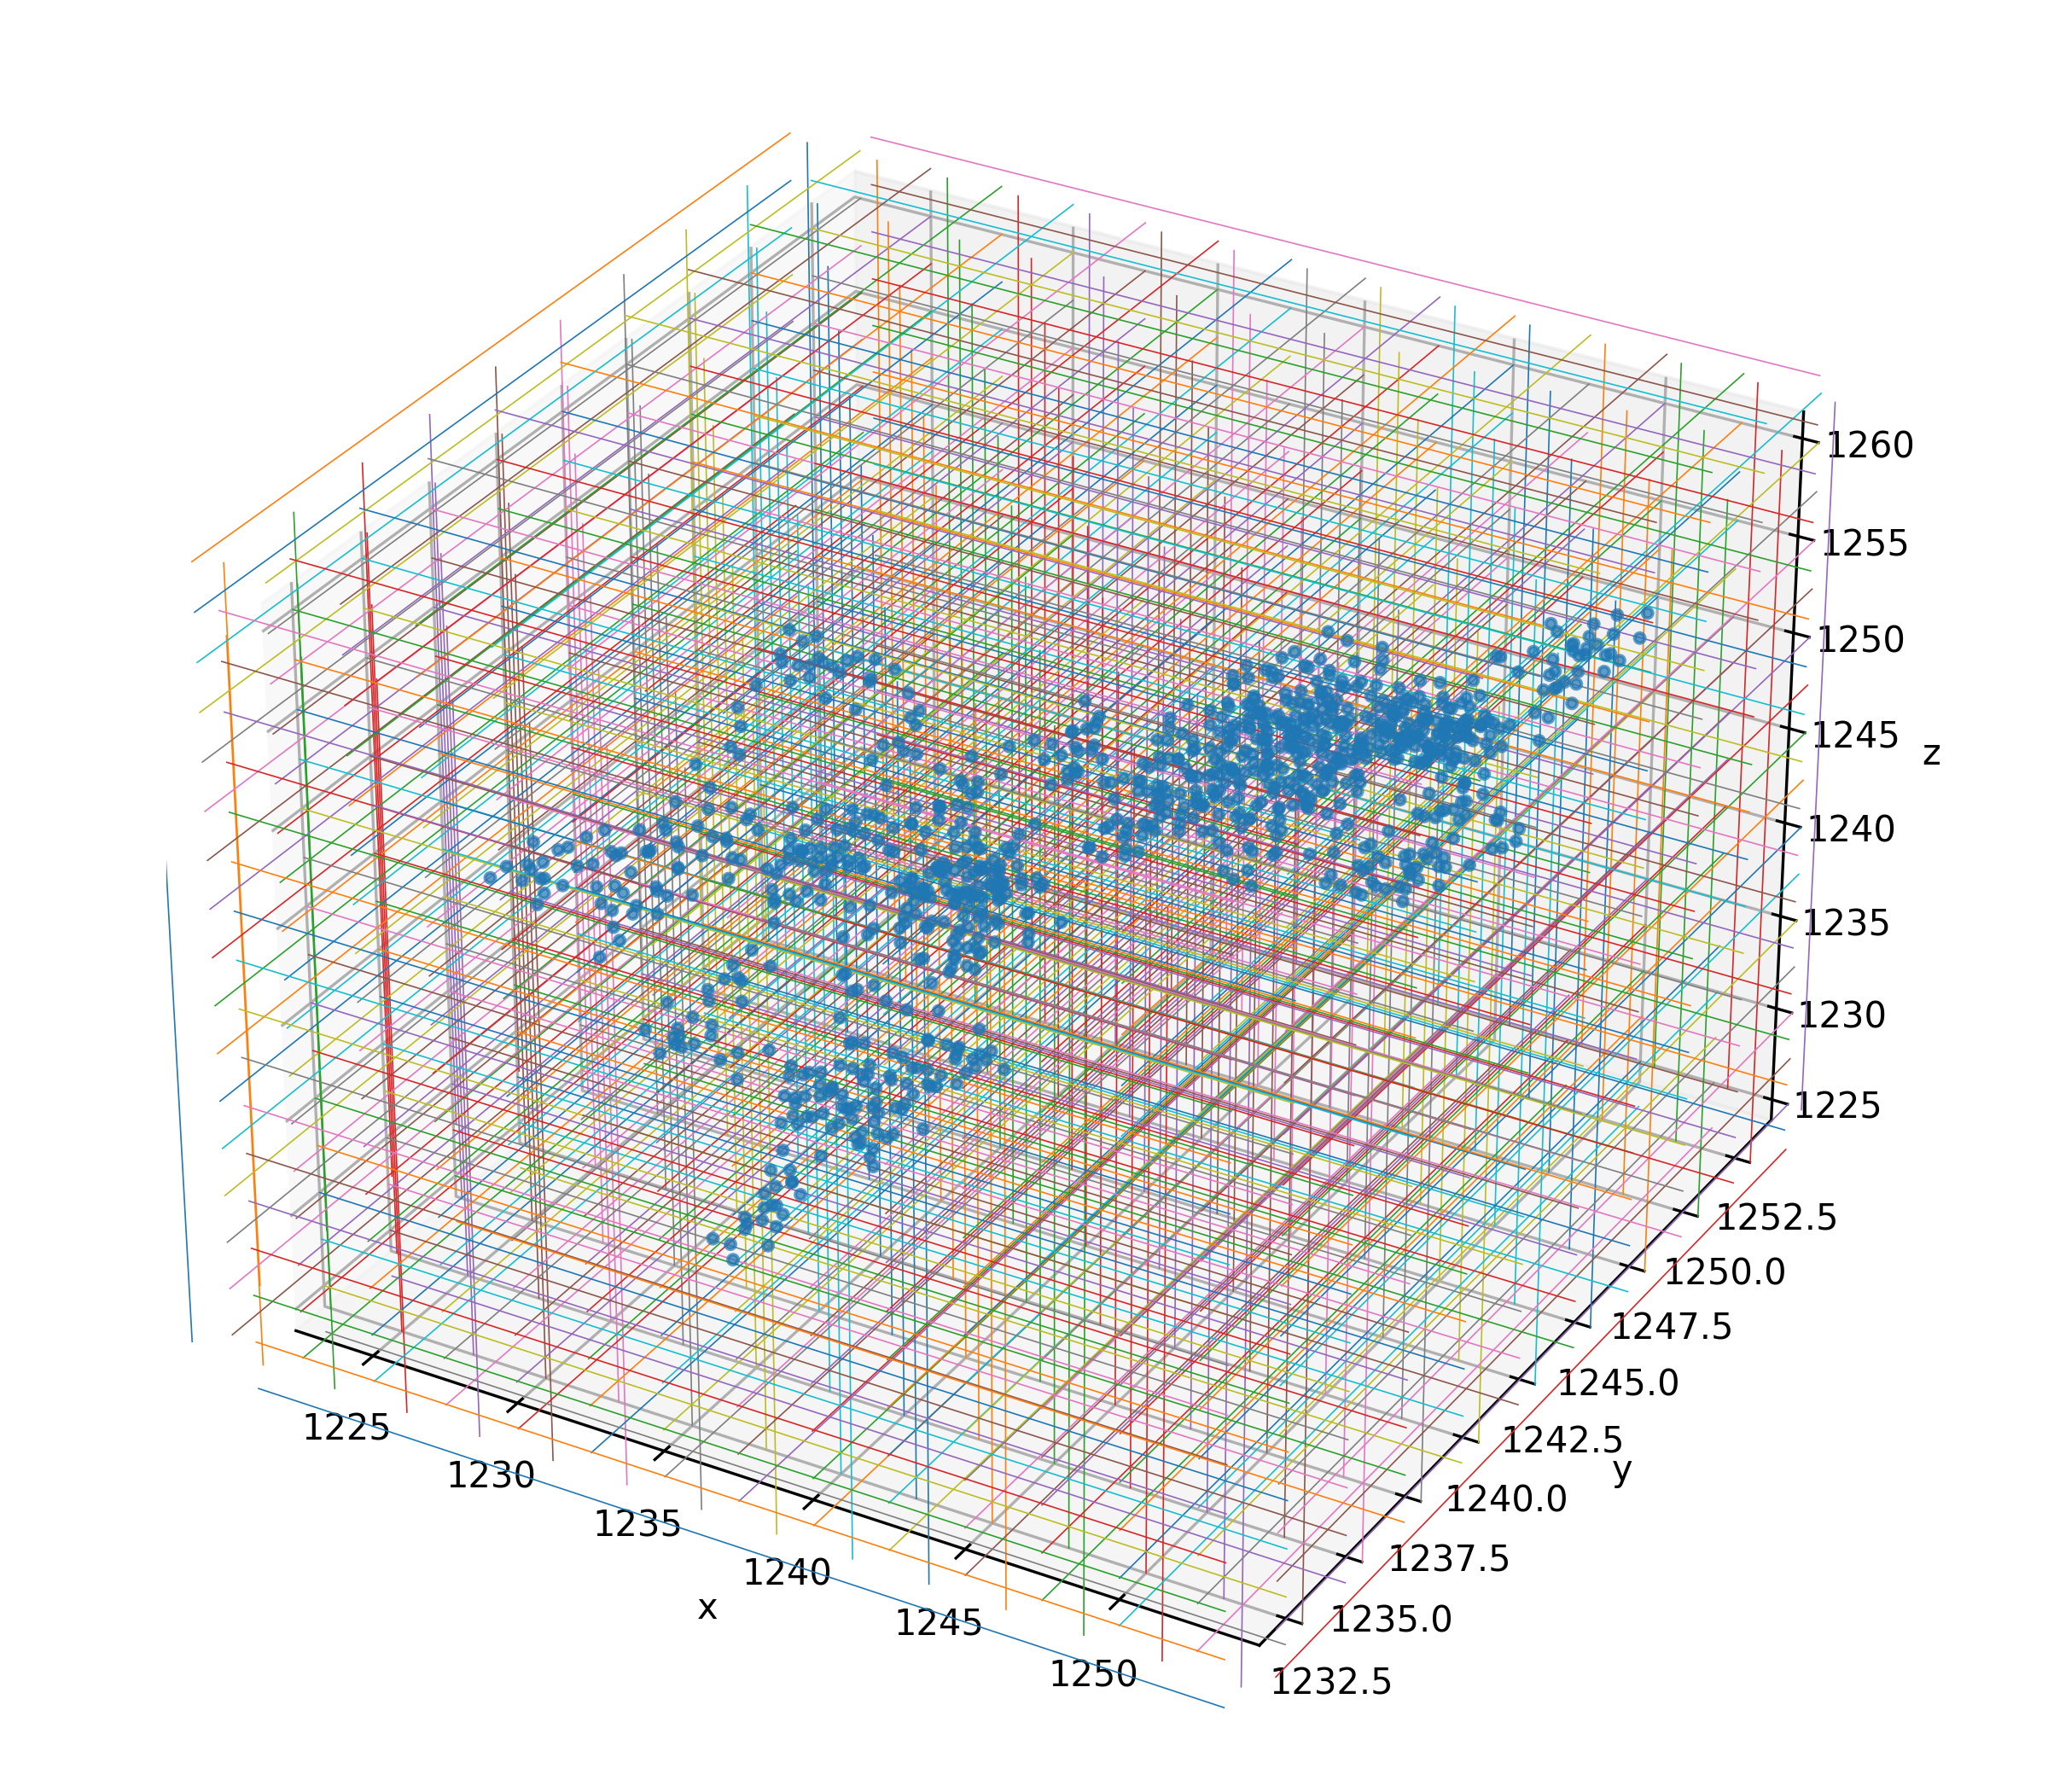
\includegraphics[width=\linewidth]{chain_overview.png}
        \caption{Overview of the atom chain within the box}
        \label{fig:chain_overview}
    \end{subfigure}
    \hfill
    \begin{subfigure}{0.48\textwidth}
        \centering
        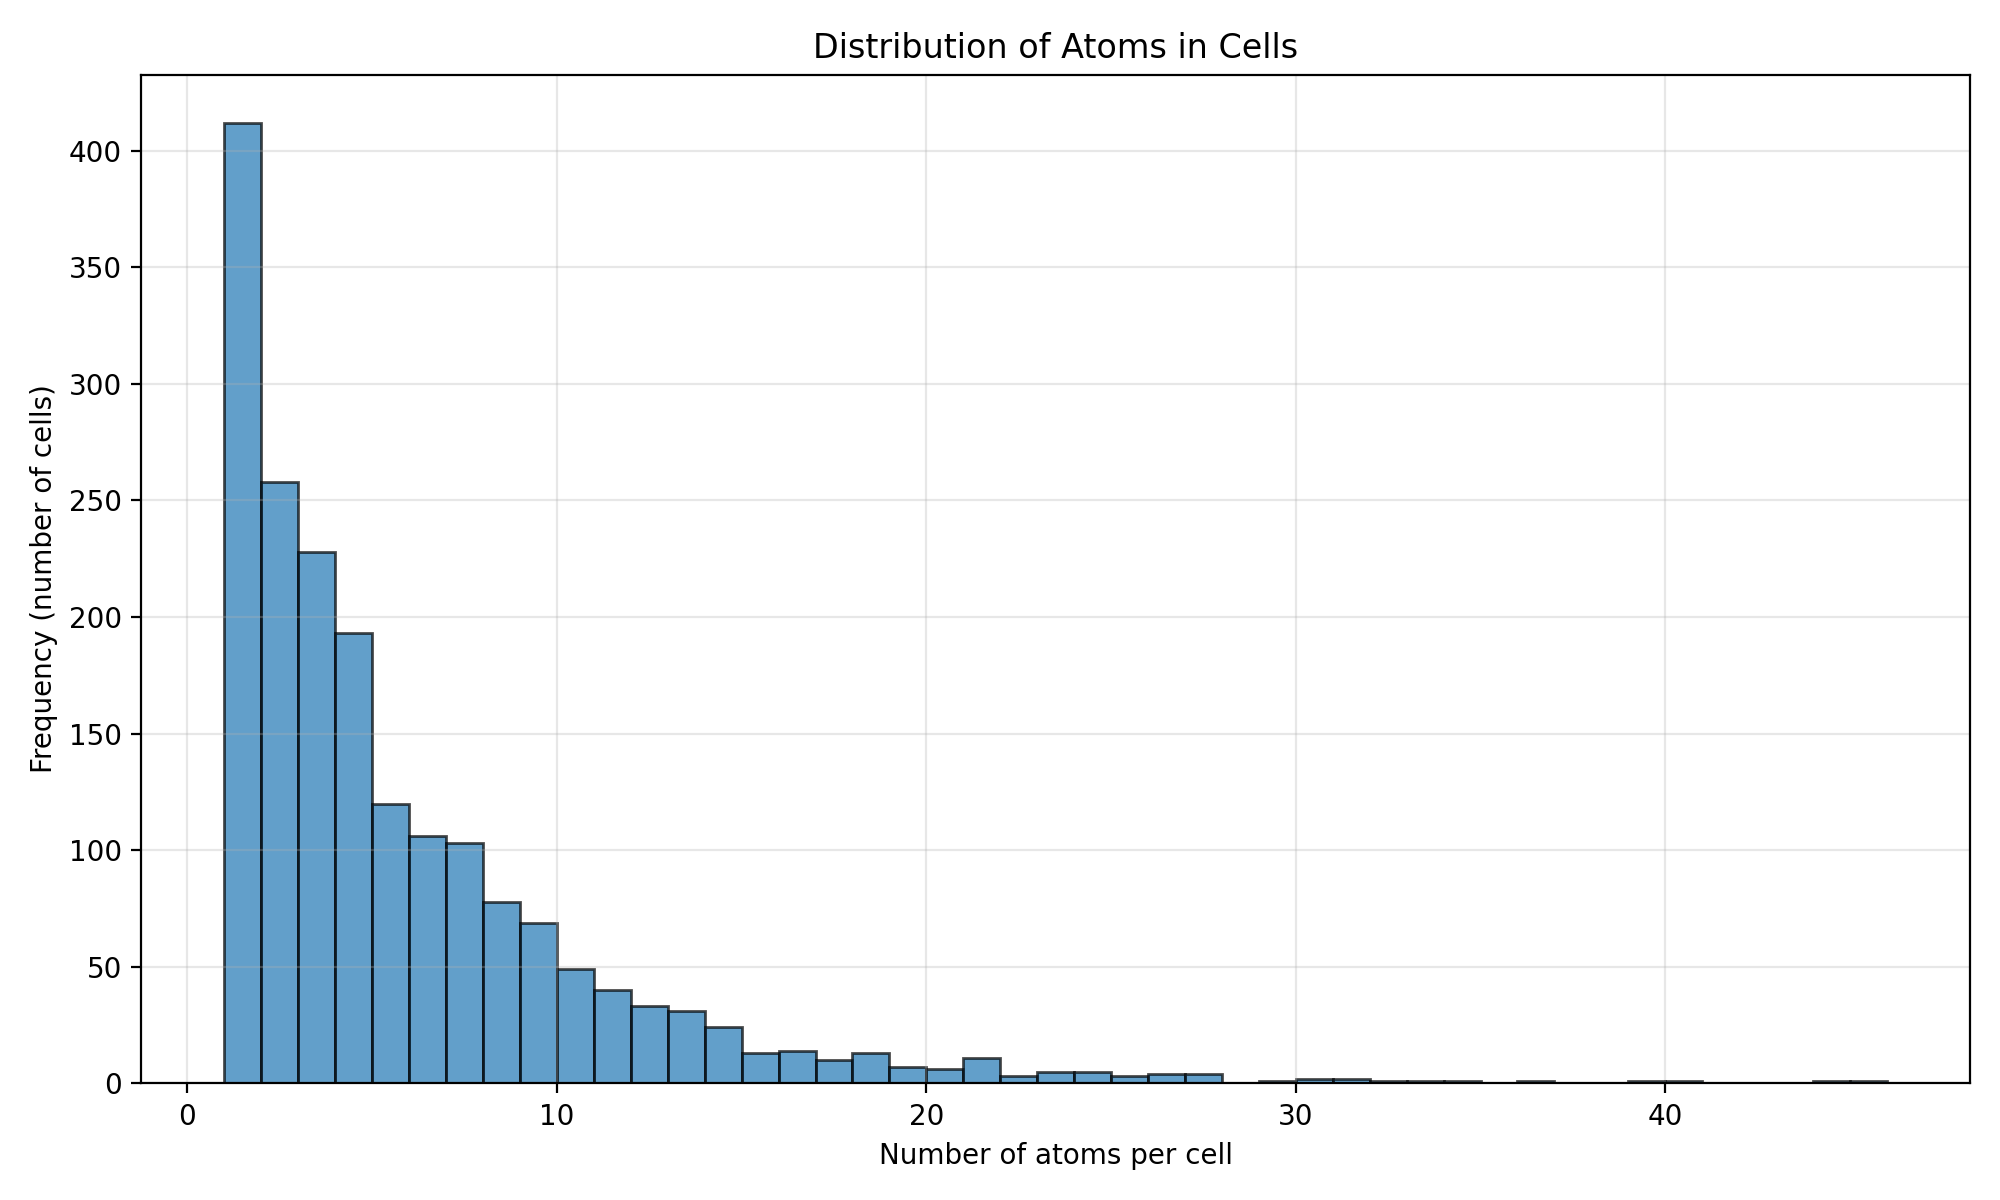
\includegraphics[width=\linewidth]{occupancy_distribution.png}
        \caption{Histogram of non-empty-cell atom count}
        \label{fig:cell_histo}
    \end{subfigure}

    \caption{Discovery of the sparse property of the cells}
\end{figure}

When developing the algorithm, we notice that a problem: If the cell size is set too large, most of the atoms will be in several cells. In this case, we will have minimal benefit from this cutoff strategy since the computation won't save a lot. However, when the cell size is small, the memory requirement to store all of number of atoms per cell array for the prefix sum and quick access of the neighbors will be very large. For $1000*1000*1000$ cells, it will need about 8GiB memory which is too stressful for the device. Also, from Figure~\ref{fig:chain_overview}, we can see that most of cells are empty and the chain is collapsed within a small area. The distribution on the right\ref{fig:cell_histo} shows that most of the occupied cells (1855 cells out of 1,000,000,000 cells are non-empty) also contain small number of atoms. So instead of wasting memory to store the sparse cells, we decide to make the use of a similar strategy as the Compressed Sparse Row as we discuss in the lecture.

Our idea is to store only the non-empty cells instead of all cells in the simulation domain. This strategy is mainly in the second stage and shown in Algorithm~\ref{algo:compact_cell_list}. After sorting the atom labels, we use \texttt{cp.unique} to obtain the existing cell labels and the number of atoms in each occupied cell. Then, we build a compact \texttt{cell\_start} array using a prefix sum over these counts. This is similar to the Compressed Sparse Row format, where only the non-empty entries are stored.

This optimization reduces memory usage when the cell grid is very sparse. Instead of allocating an array with size equal to the total number of cells, the algorithm only allocates storage proportional to the number of occupied cells which are ensured to be smaller than the number of atoms. This is especially helpful when the cell size is small and the total number of possible cells becomes very large.

\begin{algorithm}
\caption{Build Compact Cell Index Structure}\label{algo:compact_cell_list}
\begin{algorithmic}[1]
\State $\texttt{unique\_labels}, \texttt{counts\_unique} \gets \texttt{unique}(\texttt{labels\_sorted})$

\State $\texttt{cell\_start} \gets \texttt{zeros}(\texttt{size}(\texttt{unique\_labels}) + 1)$ \Comment{Rather than $\texttt{dim}*\texttt{dim}*\texttt{dim}+1$}
\State $\texttt{cell\_start}[0] \gets 0$
\State $\texttt{cell\_start}[1:] \gets \texttt{cumsum}(\texttt{counts\_unique})$
\end{algorithmic}
\end{algorithm}

In the force computation stage, this compact representation introduces extra lookup cost shown in the Kernel\ref{algo:neighbor_check}. For each neighboring cell, the kernel needs to search through \texttt{unique\_labels} to determine whether that cell exists. If the cell is empty, it is skipped. If the cell is occupied, the corresponding range in \texttt{cell\_start} gives the atom indices for that cell. Although this adds some overhead, the cost is small compared with the significant reduction in memory usage.

\begin{algorithm}
\caption{Check Whether Neighbor Cell Exists}\label{algo:neighbor_check}
\begin{algorithmic}[1]
\For{each index $i$ in \texttt{unique\_labels}}
    \If{$\texttt{unique\_labels}[i] = \texttt{label}$}
        \State Return $i$
    \ElsIf{$\texttt{unique\_labels}[i] > \texttt{label}$}
        \State Return $-1$
    \EndIf
\EndFor

\State Return $-1$

\end{algorithmic}
\end{algorithm}

After implementing this strategy, we were able to increase the cell grid size to $1000 \times 1000 \times 1000$ for a system with 10,000 atoms. Before this optimization, even a $500 \times 500 \times 500$ cell grid caused the kernel to fail due to excessive memory requirements.

\begin{table}[h]
\centering
\caption{Summary of GPU Platforms Used for Testing}
\label{tab:gpu_platforms}
\resizebox{\textwidth}{!}{
\begin{tabular}{lcc}
\hline
\textbf{Specification} & \textbf{Google Colab} & \textbf{School Linux Cluster} \\
\hline
GPU Model & Tesla T4 & NVIDIA RTX 4000 Ada Generation \\
Driver Version & 580.82.07 & 580.65.06 \\
CUDA Version & 13.0 & 13.0 \\
GPU Memory & 15,360 MiB & 20,475 MiB \\
Power Limit & 70 W & 130 W \\
Idle Temperature & 38$^\circ$C & 29$^\circ$C \\
Idle Power Usage & 10 W & 11 W \\
Compute Mode & Default & Default \\
\hline
\end{tabular}
}
\end{table}

\section{Performance Measurements}
% Present results of performance testing and comparison to other versions.

For our experiments, we mainly measured two metrics: runtime and hardware utilization. These experiments were tested on two different platforms, as shown in Table~\ref{tab:gpu_platforms}. The runtime experiments were performed on the School Linux Cluster, while the hardware utilization experiments were performed on the Google Colab server.

\subsection{Runtime Analysis}
We measured the empirical run time of different force computation algorithms by taking the average between 4 runs after one warm-up round. As stated in Section \ref{sec:intro}, a typical commercial linear polymer has a chain length ranging from 1000 to 10000 monomers. Therefore, we measured the performance of our algorithms with N ranging from $10^3$ to $10^4$.

Using the sequential exact algorithm’s run time as a baseline, we computed the speedup achieved and plotted them against N. The plots are shown in figure \ref{fig:forcePerformance}.

\begin{figure}[h]
    \centering
    
    \begin{subfigure}{0.45\textwidth}
        \centering
        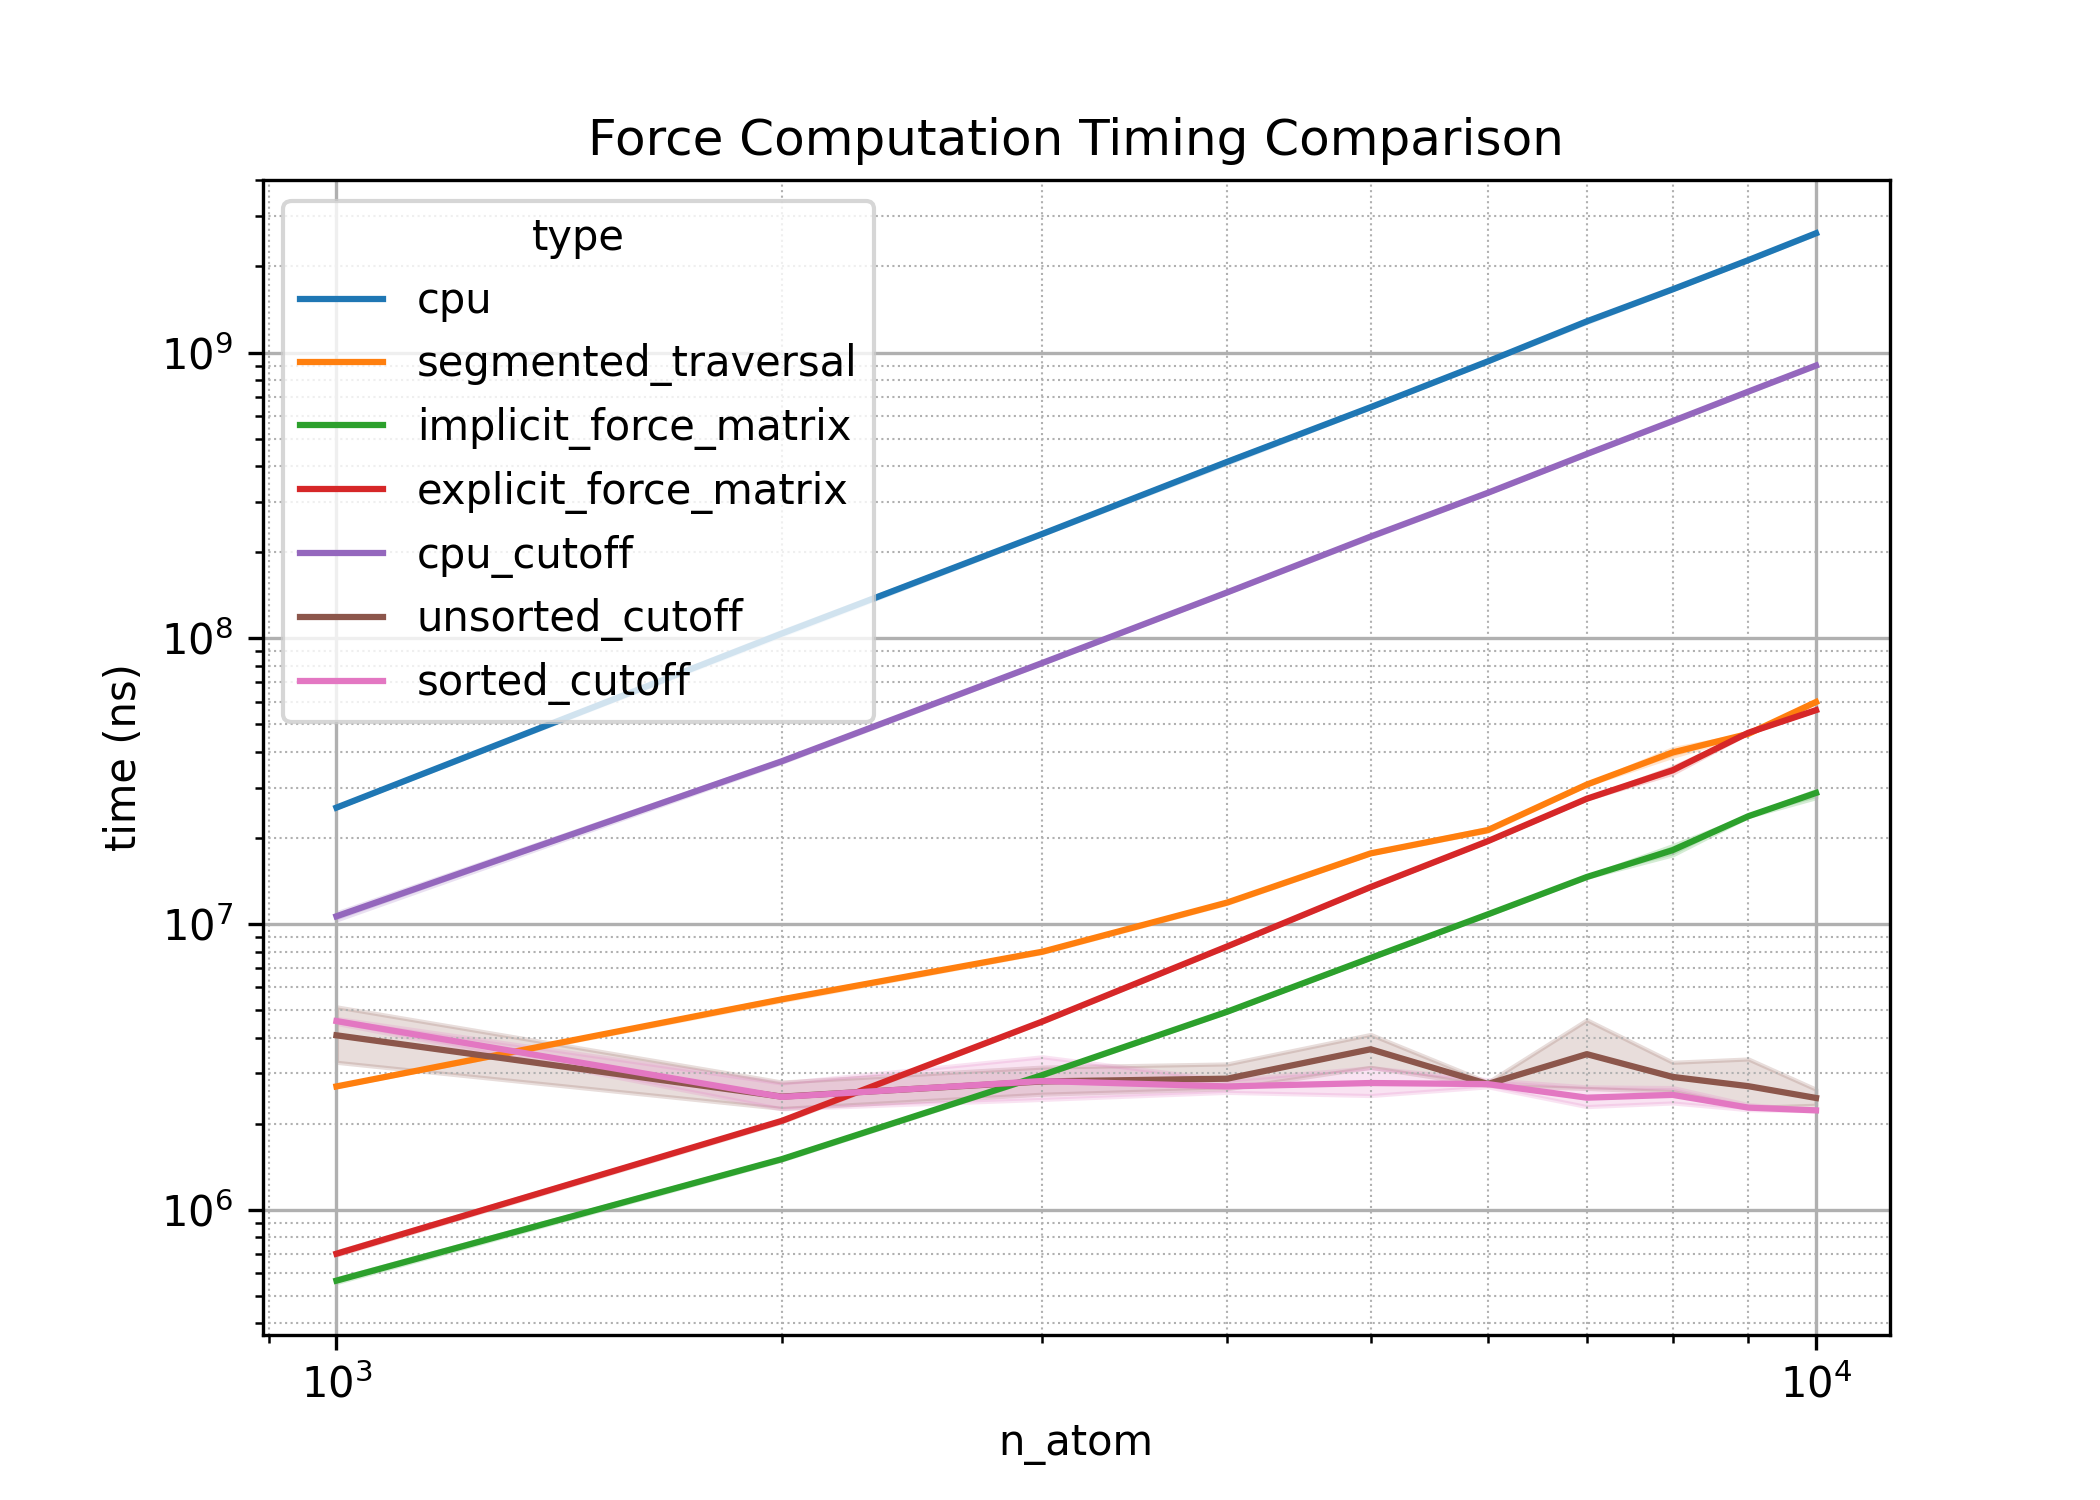
\includegraphics[width=\linewidth]{combined_timing.png}
        \caption{Timing comparisons}
    \end{subfigure}
    \hfill
    \begin{subfigure}{0.45\textwidth}
        \centering
        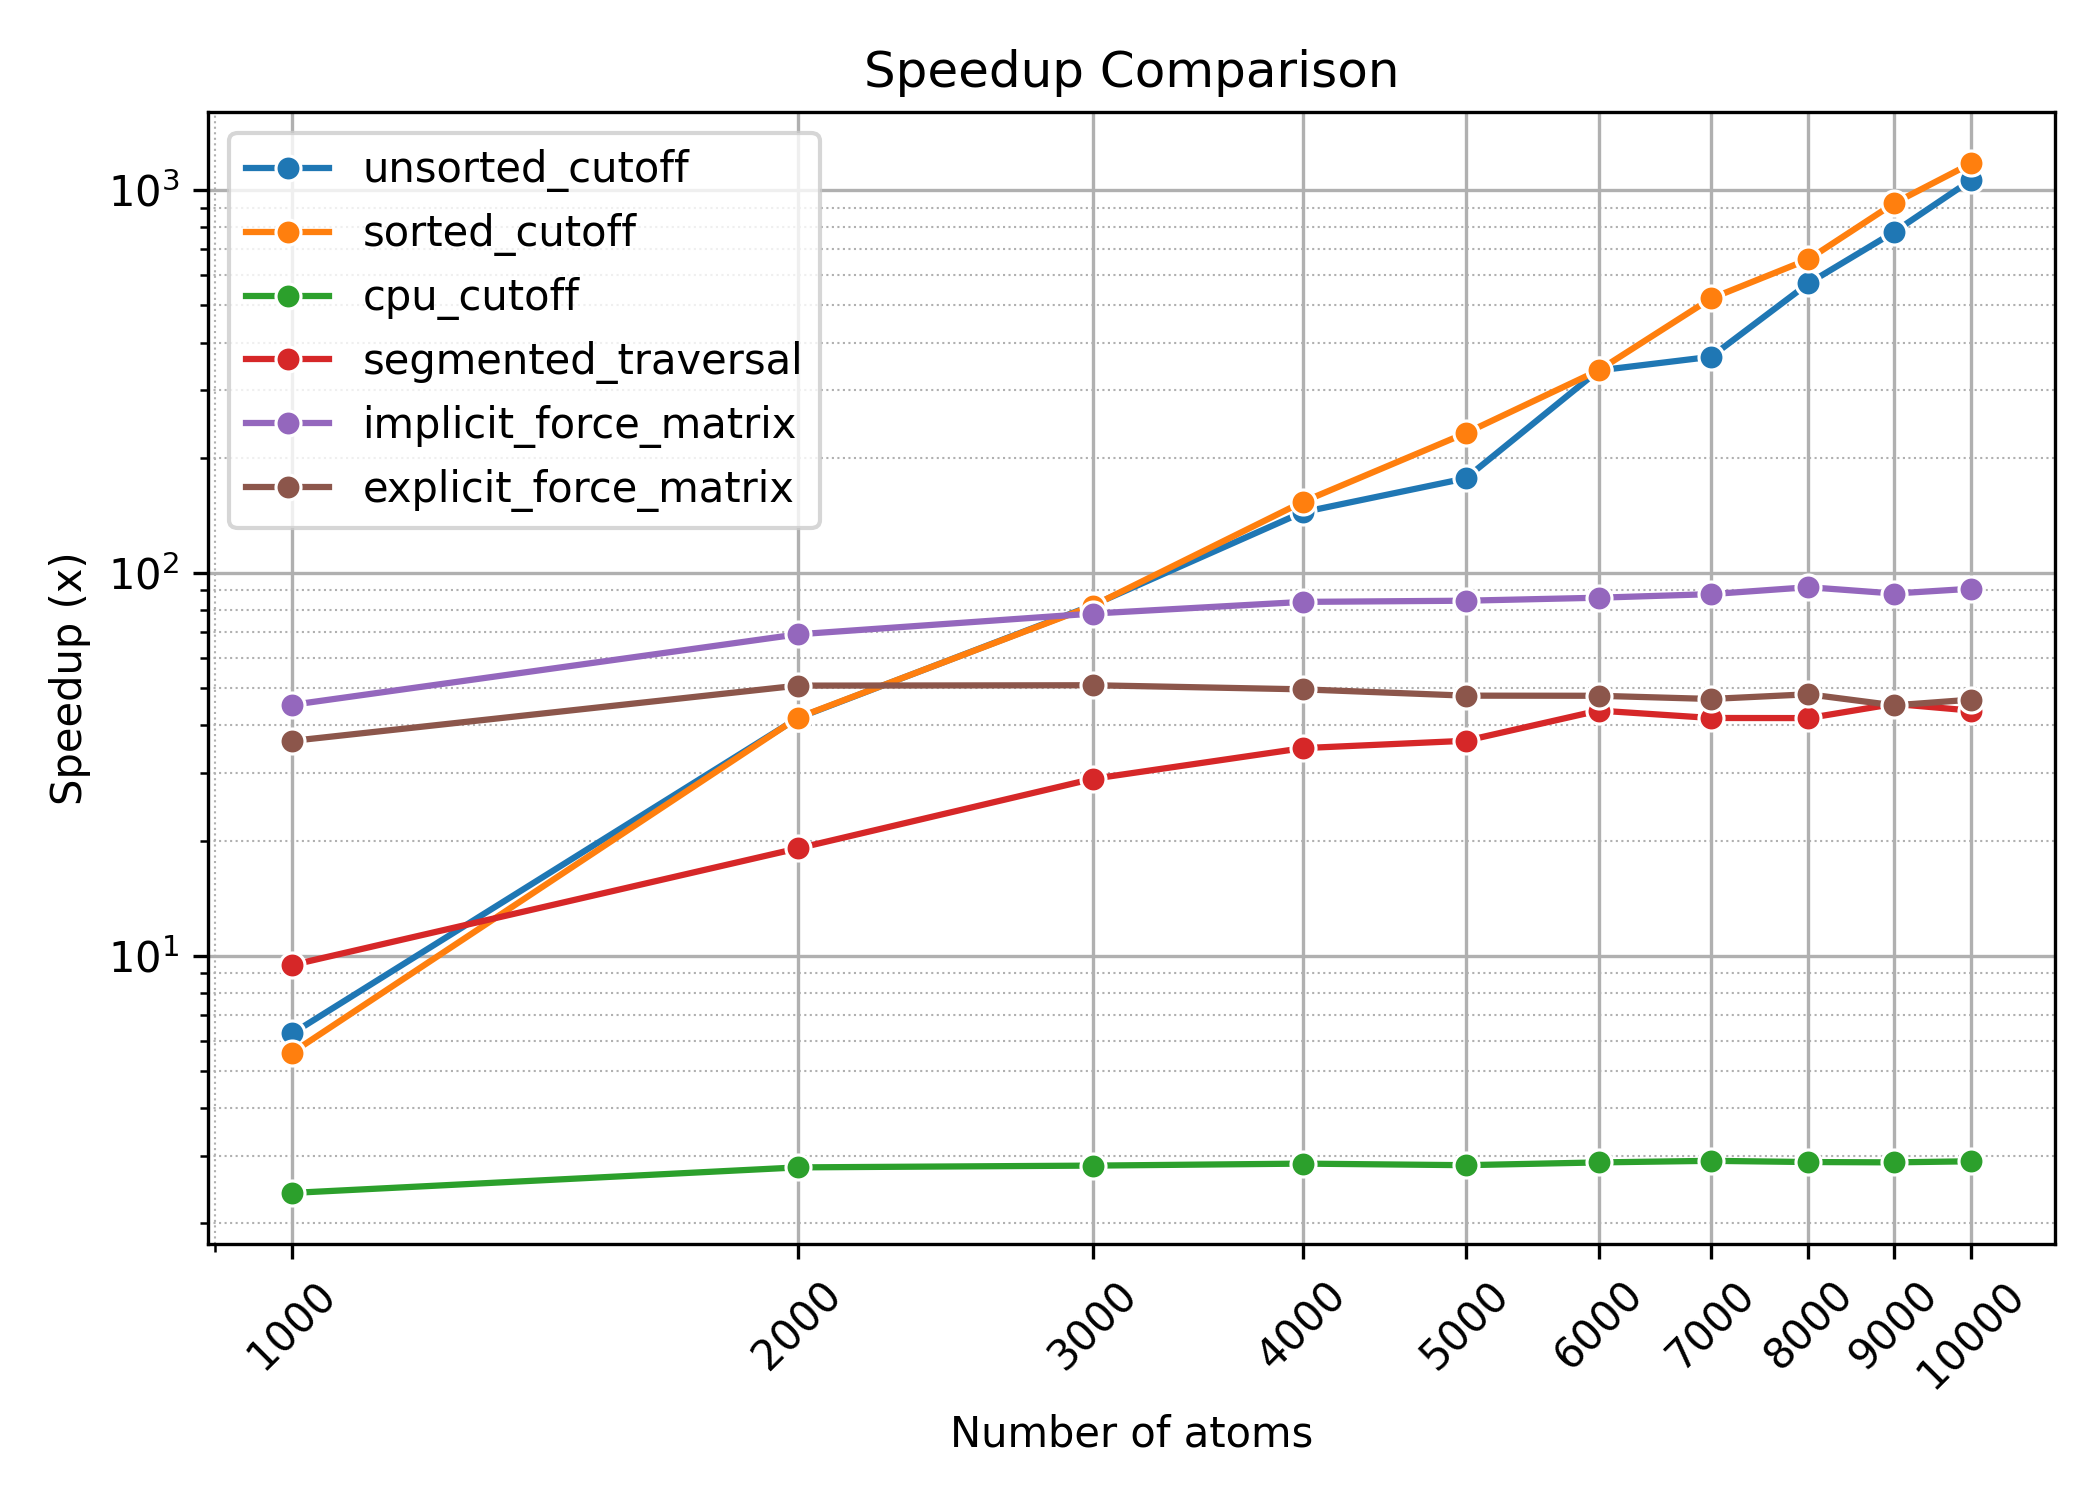
\includegraphics[width=\linewidth]{combined_speedup.png}
        \caption{Speedup comparisons}
    \end{subfigure}

    \caption{Comparisons for the force computation kernels}
    \label{fig:forcePerformance}
\end{figure}

In addition, we measured the total run time of 101-step integrations using the different force computation algorithms, and compared their speedup using the sequential exact algorithm as a baseline. The results are shown in figure \ref{fig:integrationPerformance}.

\begin{figure}[h]
    \centering
    
    \begin{subfigure}{0.45\textwidth}
        \centering
        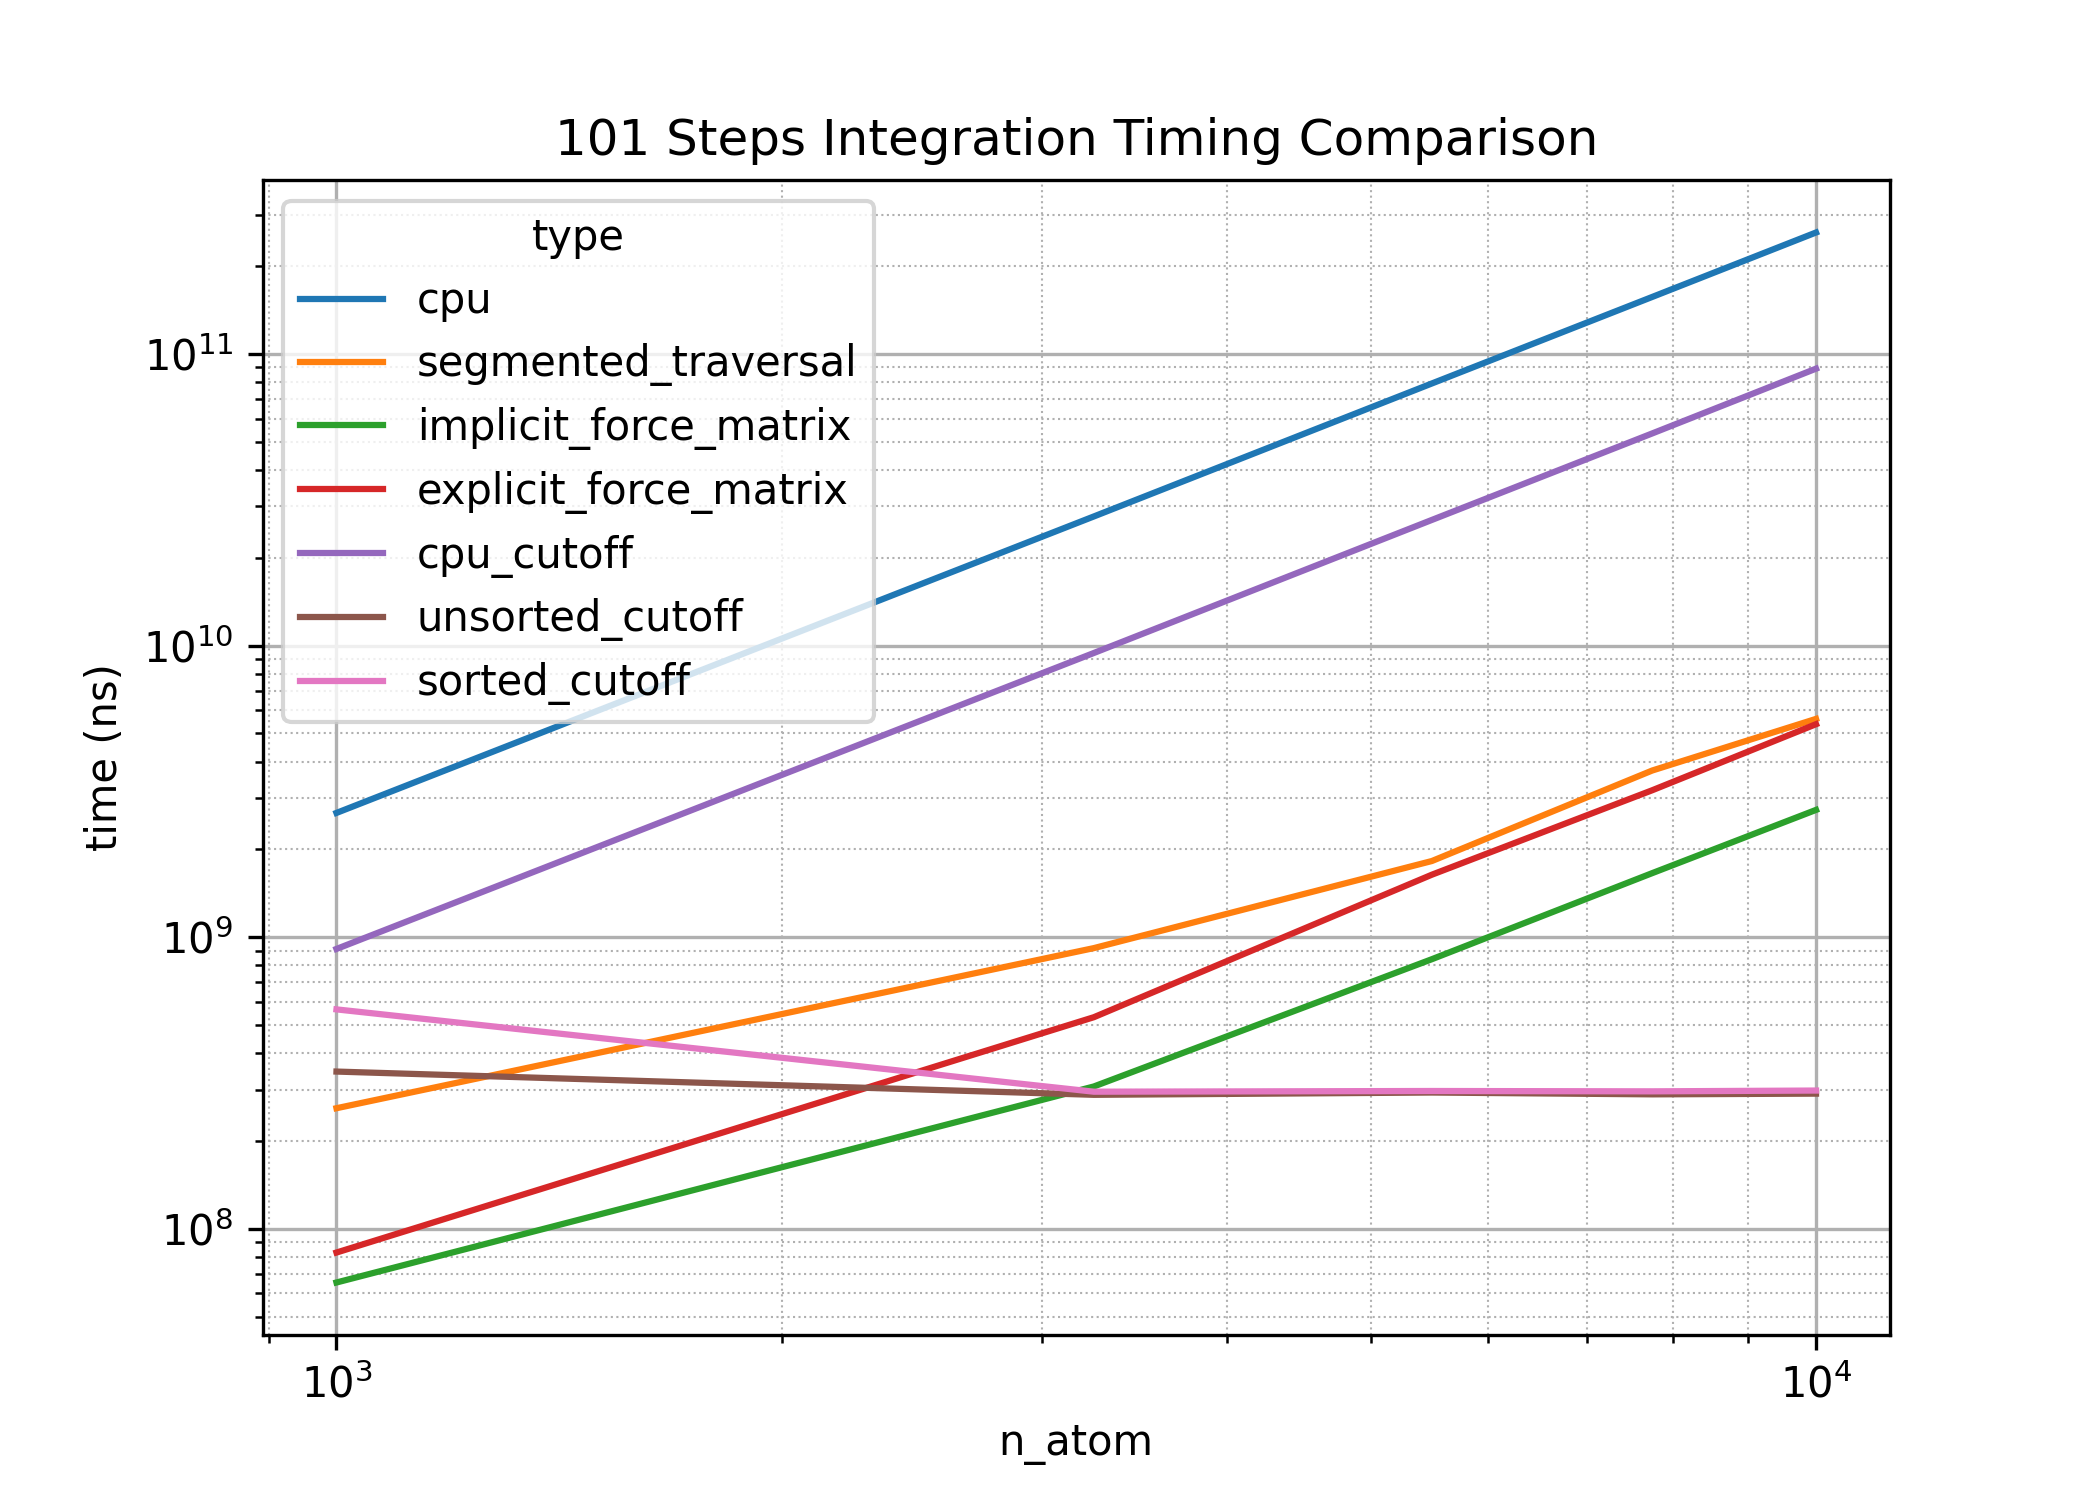
\includegraphics[width=\linewidth]{combined_101_timing.png}
        \caption{Timing comparisons}
    \end{subfigure}
    \hfill
    \begin{subfigure}{0.45\textwidth}
        \centering
        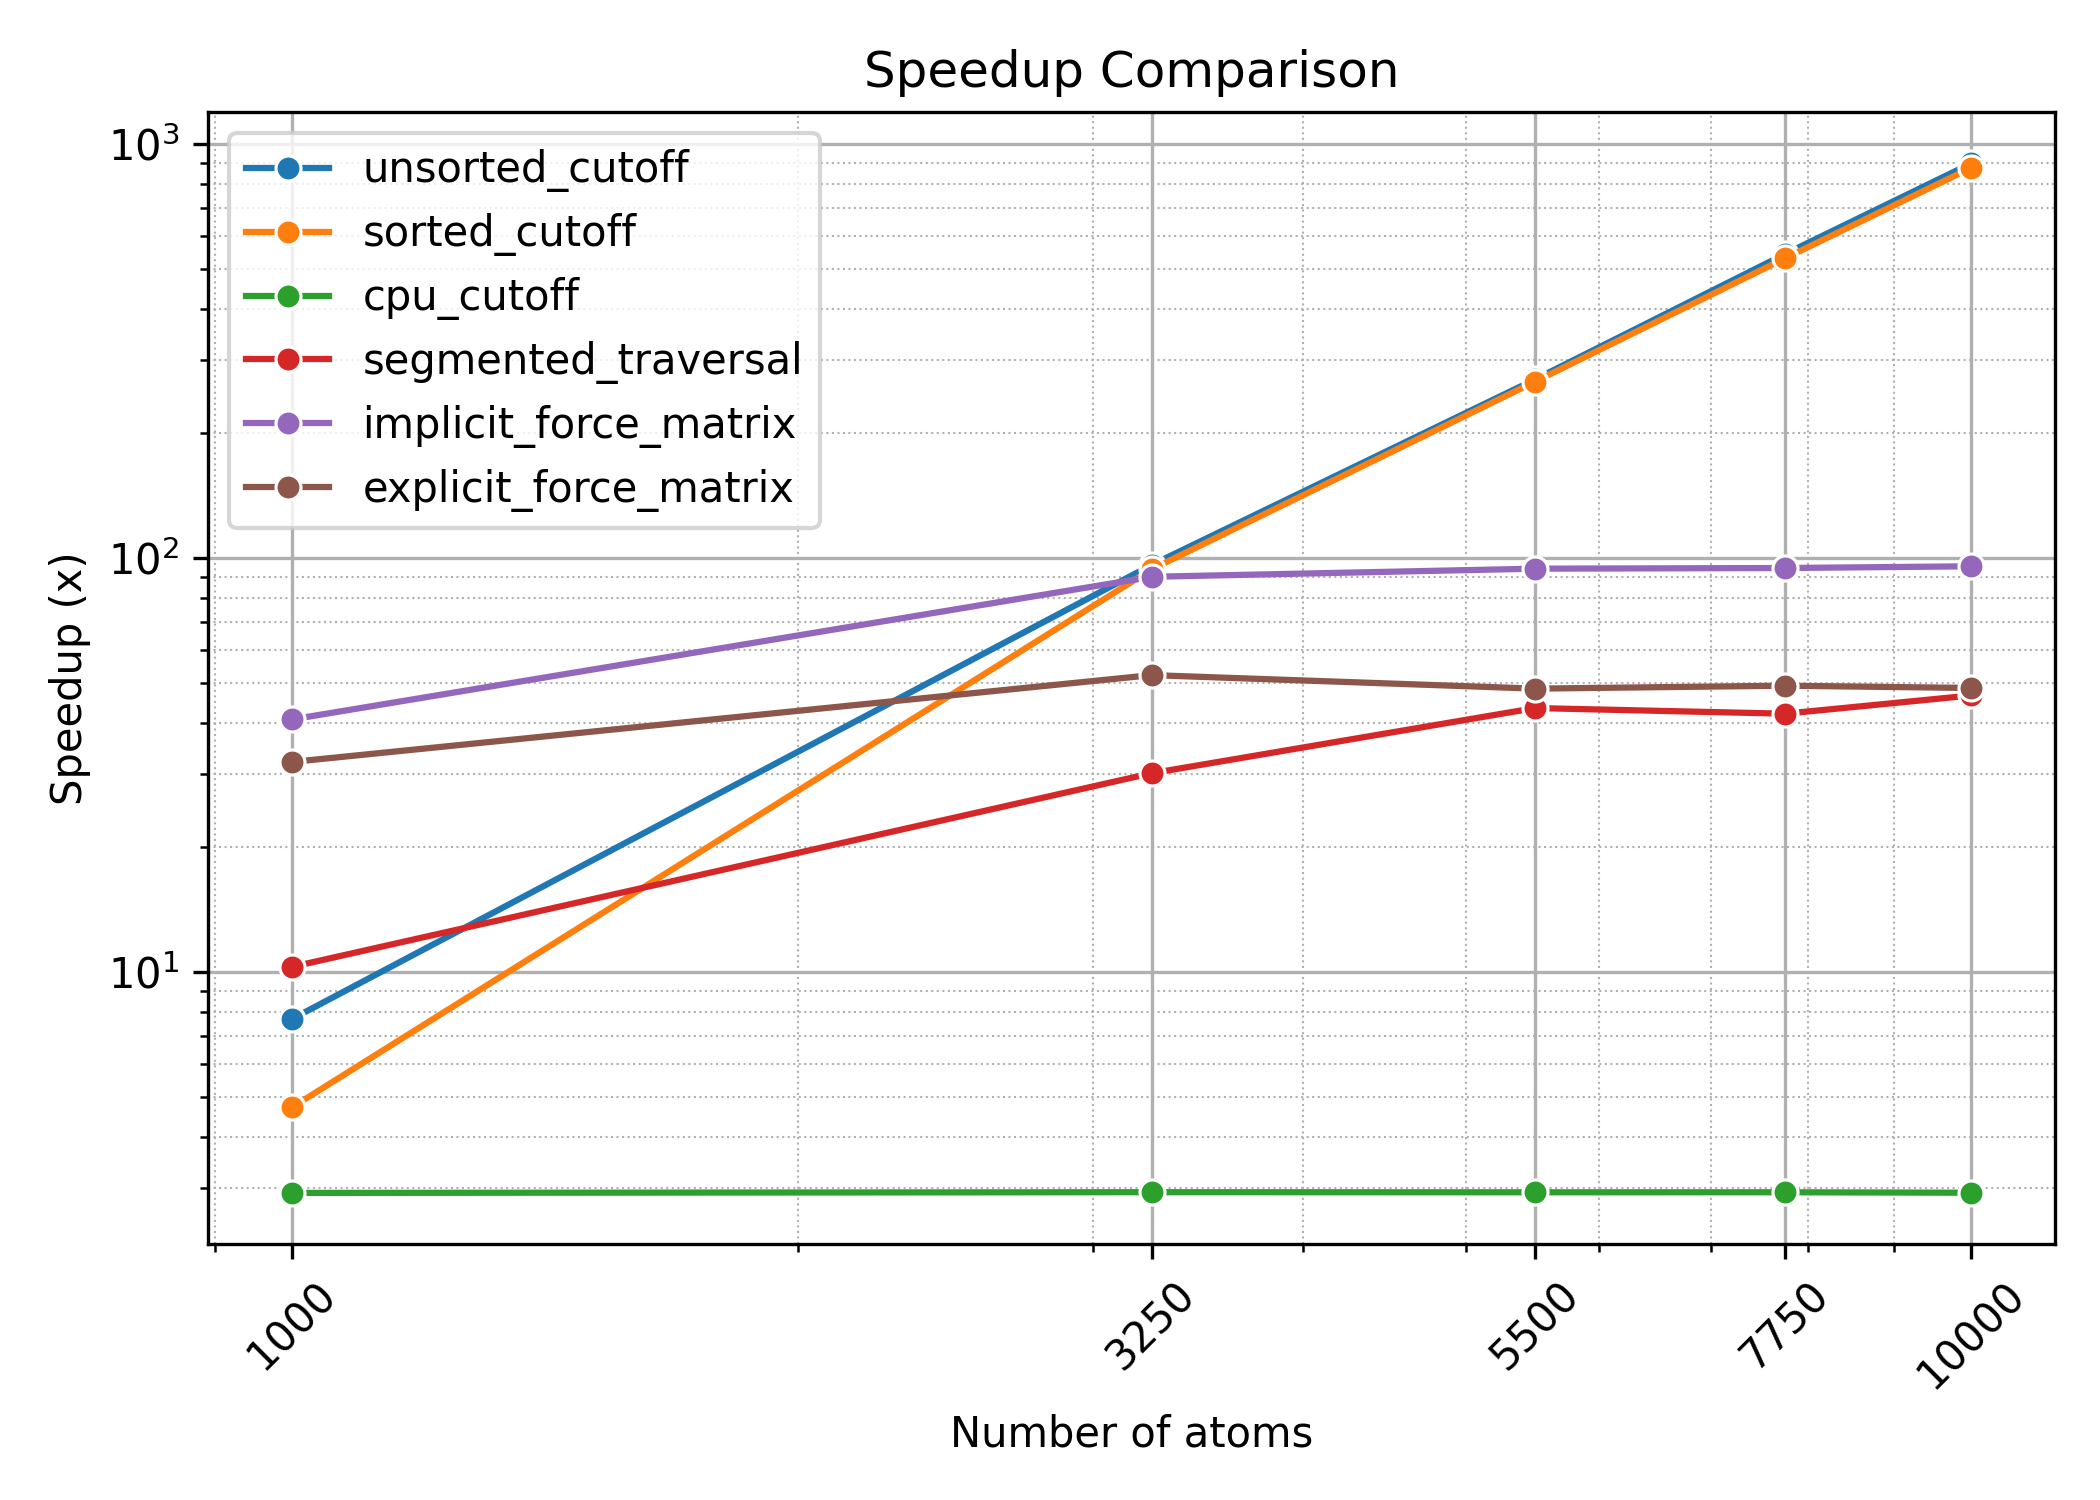
\includegraphics[width=\linewidth]{combined_101_speedup.png}
        \caption{Speedup comparisons}
    \end{subfigure}

    \caption{Comparisons for the total run time of 101-step integrations}
    \label{fig:integrationPerformance}
\end{figure}


\subsection{Hardware Analysis}

In these experiments, we selected only our custom CUDA kernels for profiling with the NVIDIA Nsight Compute profiler. This allows us to focus on the performance of the kernels we implemented, instead of including extra CuPy or library kernels that are not part of the main optimization. We used the roofline model because it provides a clear view of whether each kernel is mainly limited by computation or memory bandwidth. For profiling, we ran each case for 5 simulation steps. This was enough to capture the main hardware utilization behavior, while avoiding unnecessary profiling overhead. Using more steps would significantly increase the total runtime but would not provide much additional useful information for comparing the kernels. The results are summarized in Table~\ref{tab:ncu_kernel_summary} and Table~\ref{tab:ncu_kernel_summary_10000}.

\begin{table}[h]
\centering
\caption{Nsight Compute Summary for Major Kernels with 1000 Atoms}
\label{tab:ncu_kernel_summary}
\resizebox{\textwidth}{!}{
\begin{tabular}{lcccccl}
\hline
\textbf{Kernel} & \textbf{Grid} & \textbf{Block} & \textbf{Duration} & \textbf{SM Throughput} & \textbf{Memory Throughput} \\
\hline

\texttt{calc\_force\_matrix} 
& $528$ & $32$ & $1.49~ms$ & $83.38\%$ & $1.36\%$ \\

\texttt{calc\_force\_matrix\_explicit} 
& $976$ & $512$ & $1.70~ms$ & $86.44\%$ & $2.54\%$ \\

\texttt{force\_mat\_sum} 
& $1000$ & $512$ & $244.22~\mu s$ & $53.08\%$ & $41.56\%$ \\

\texttt{calc\_force\_cutoff\_gpu\_unsorted} 
& $8$ & $128$ & $2.20~ms$ & $14.40\%$ & $0.59\%$ \\

\texttt{atom\_label\_kernel} 
& $8$ & $128$ & $15.04~\mu s$ & $13.47\%$ & $0.80\%$ \\

\texttt{calc\_force\_cutoff\_gpu\_sorted} 
& $8$ & $128$ & $7.53~ms$ & $10.80\%$ & $0.18\%$ \\

\hline
\end{tabular}
}
\end{table}

\begin{table}[h]
\centering
\caption{Nsight Compute Summary for Major Kernels with 10,000 Atoms}
\label{tab:ncu_kernel_summary_10000}
\resizebox{\textwidth}{!}{
\begin{tabular}{lcccccl}
\hline
\textbf{Kernel} & \textbf{Grid} & \textbf{Block} & \textbf{Duration} & \textbf{SM Throughput} & \textbf{Memory Throughput} \\
\hline
\texttt{calc\_force\_matrix}
& $49141$ & $32$ & $129.37~ms$ & $89.45\%$ & $1.55\%$ \\

\texttt{calc\_force\_matrix\_explicit}
& $97647$ & $512$ & $161.51~ms$ & $89.45\%$ & $2.85\%$ \\

\texttt{force\_mat\_sum}
& $10000$ & $512$ & $80.79~ms$ & $11.34\%$ & $89.13\%$ \\

\texttt{calc\_force\_cutoff\_gpu\_unsorted}
& $79$ & $128$ & $89.22~\mu s$ & $79.20\%$ & $1.86\%$ \\

\texttt{atom\_label\_kernel}
& $79$ & $128$ & $26.43~\mu s$ & $74.78\%$ & $3.29\%$ \\

\texttt{calc\_force\_cutoff\_gpu\_sorted}
& $79$ & $128$ & $68.48~\mu s$ & $77.85\%$ & $1.57\%$ \\
\hline
\end{tabular}
}
\end{table}

\section{Results}
% Summarize findings and outcomes.

\subsection{Correctness}
Correctness of the force computation kernels are checked by comparing the forces calculated by the GPU kernels to those calculated by CPU code, using the \texttt{np.allclose} function. However, it is expected that the trajectories will significantly deviate between the different methods during integration. Since floating point addition is not commutative, the different operation sequence due to parallelization and grid scheduling will almost certainly lead to small deviations in the forces computed in each step. During the thousands of steps of integration, these errors accumulate and get amplified, leading to completely different positions at the end of the simulation.

Therefore, we further tested the ensemble properties of the system at the end of the simulation. Specifically, we examined the potential energy (figure \ref{fig:pe_comp}) and radial distribution function (RDF)  of our systems at the last 10 frames of a 1000-step integration. Potential energy measures the thermodynamics properties of the system, while the RDF describes the spatial distribution of the particles.

As seen in figure \ref{fig:pe_comp}, the exact kernels have very similar potential energies that overlap with each other on the plot, while the cutoff kernel differs both significantly from the CPU code result and from the exact results. In figure \ref{fig:rdf_comp}, we found that the exact kernels again produce similar results. While the cutoff kernel results in a similar RDF as the CPU results, they differ significantly from the exact results.

We conclude that the exact kernels produce the correct system behaviors despite having different particle trajectories due to floating point rounding errors. However, both the cutoff CPU code and the cutoff kernel deviate from the expected behavior. While the deviation between the cutoff CPU code and the kernel can be explained by floating point errors, their deviation from the exact results are rooted in chemical principles. One explanation is that the conventional cutoff of $2.5\sigma$ is insufficient to capture all the necessary interactions in our system, which is a sparse simulation system without solvent to mediate interactions. Another explanation could be that the bonds themselves stretch beyond the cutoff distance, which leads to incorrect cutoff of the bonded interactions. Although this would be an anomoly given the large spring constant, the effects could propagate through the simulation and lead to completely different results.

\begin{figure}[h]
    \centering
    
    \begin{subfigure}{0.45\textwidth}
        \centering
        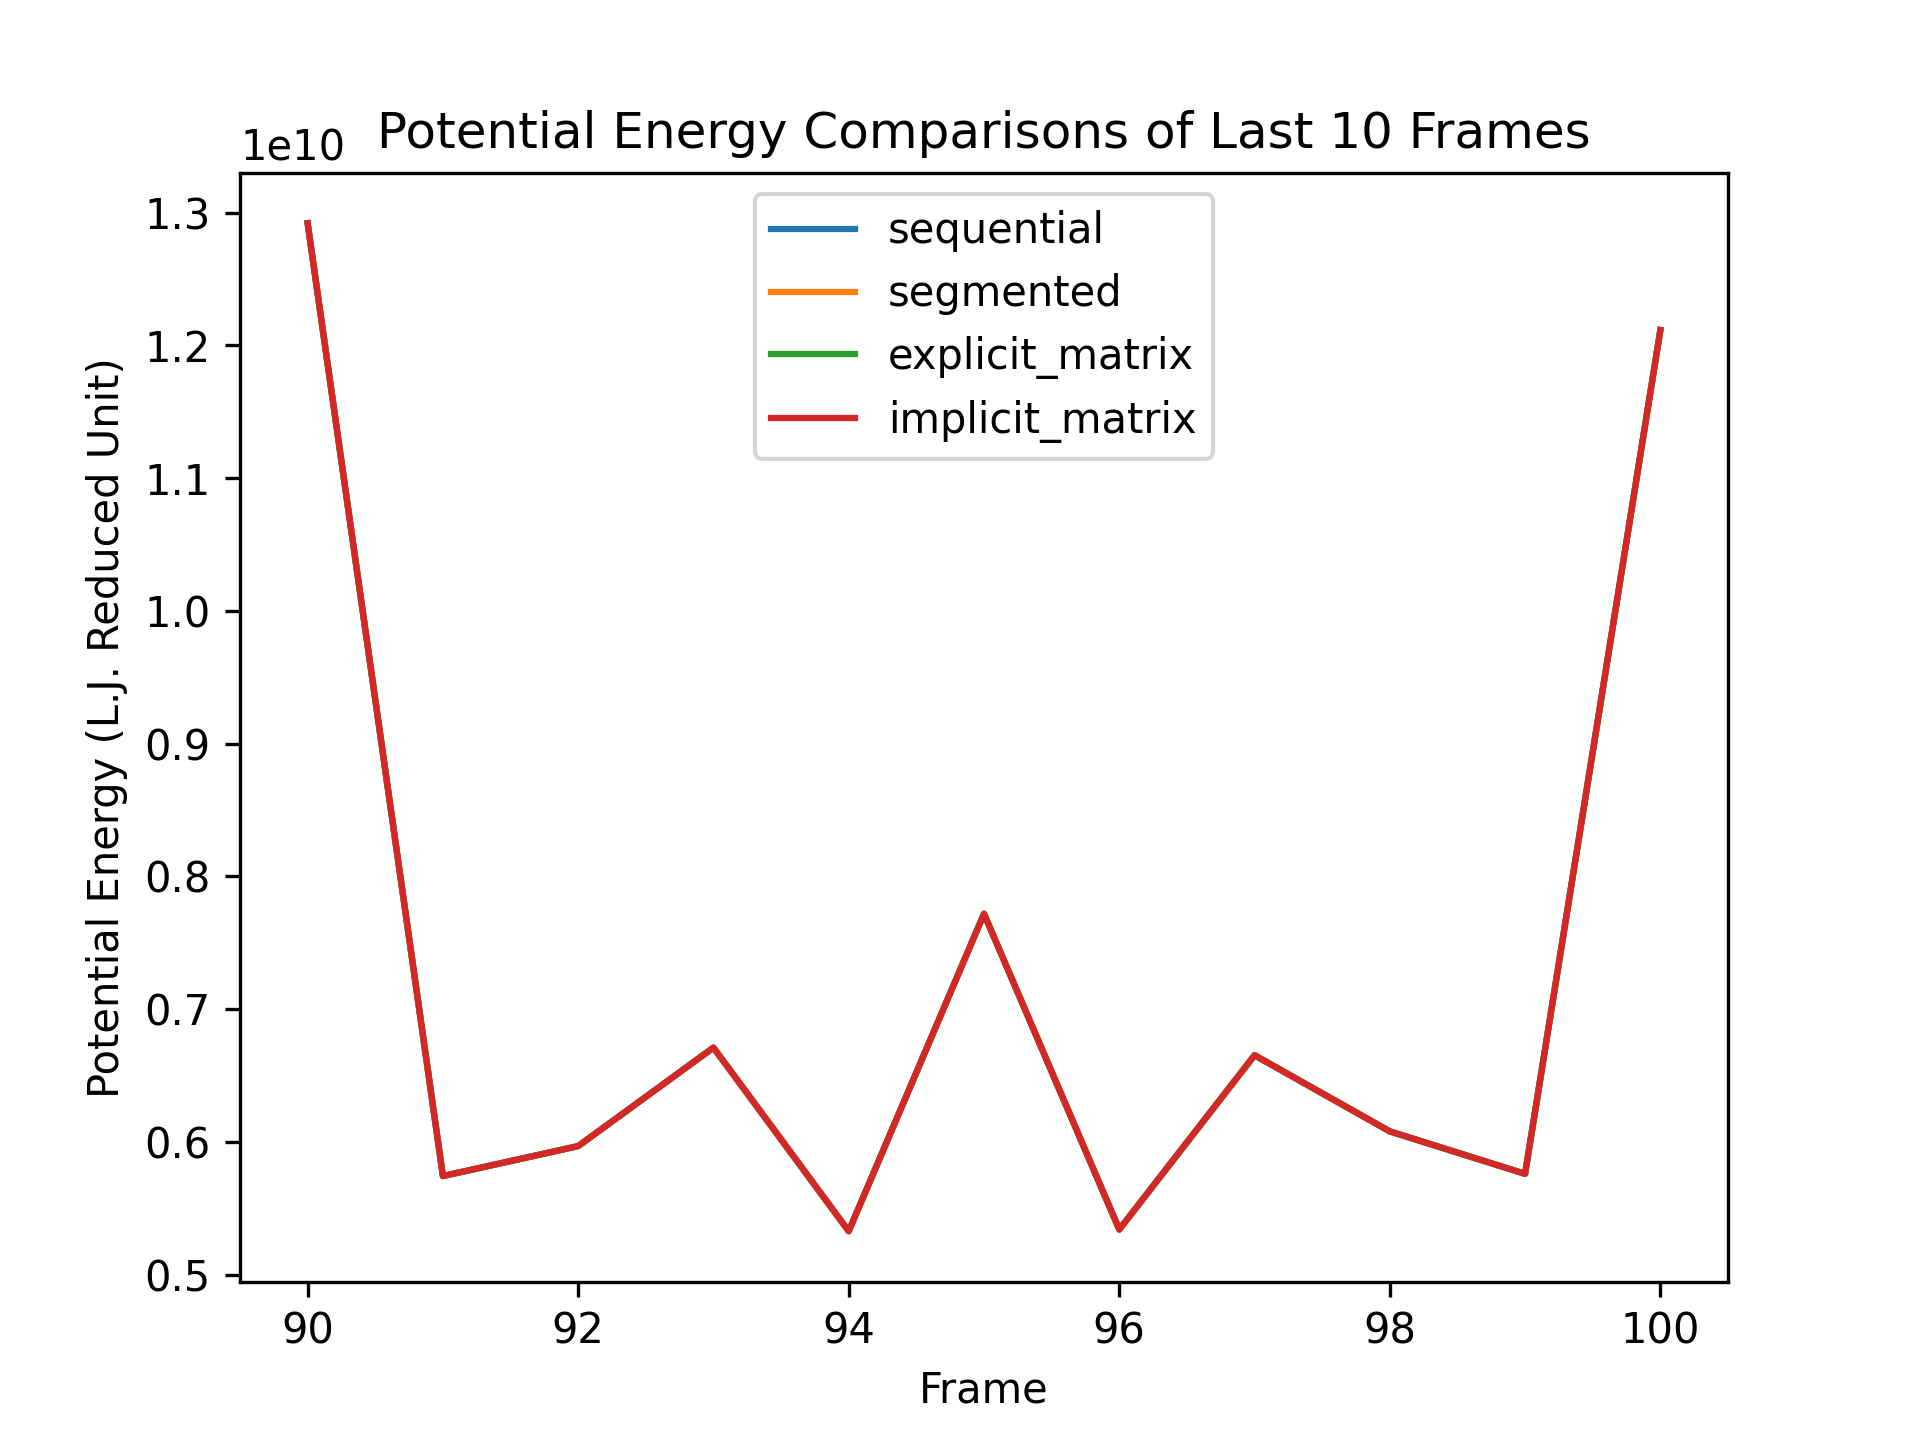
\includegraphics[width=\linewidth]{pe.png}
        \caption{Exact Kernel Comparisons}
    \end{subfigure}
    \hfill
    \begin{subfigure}{0.45\textwidth}
        \centering
        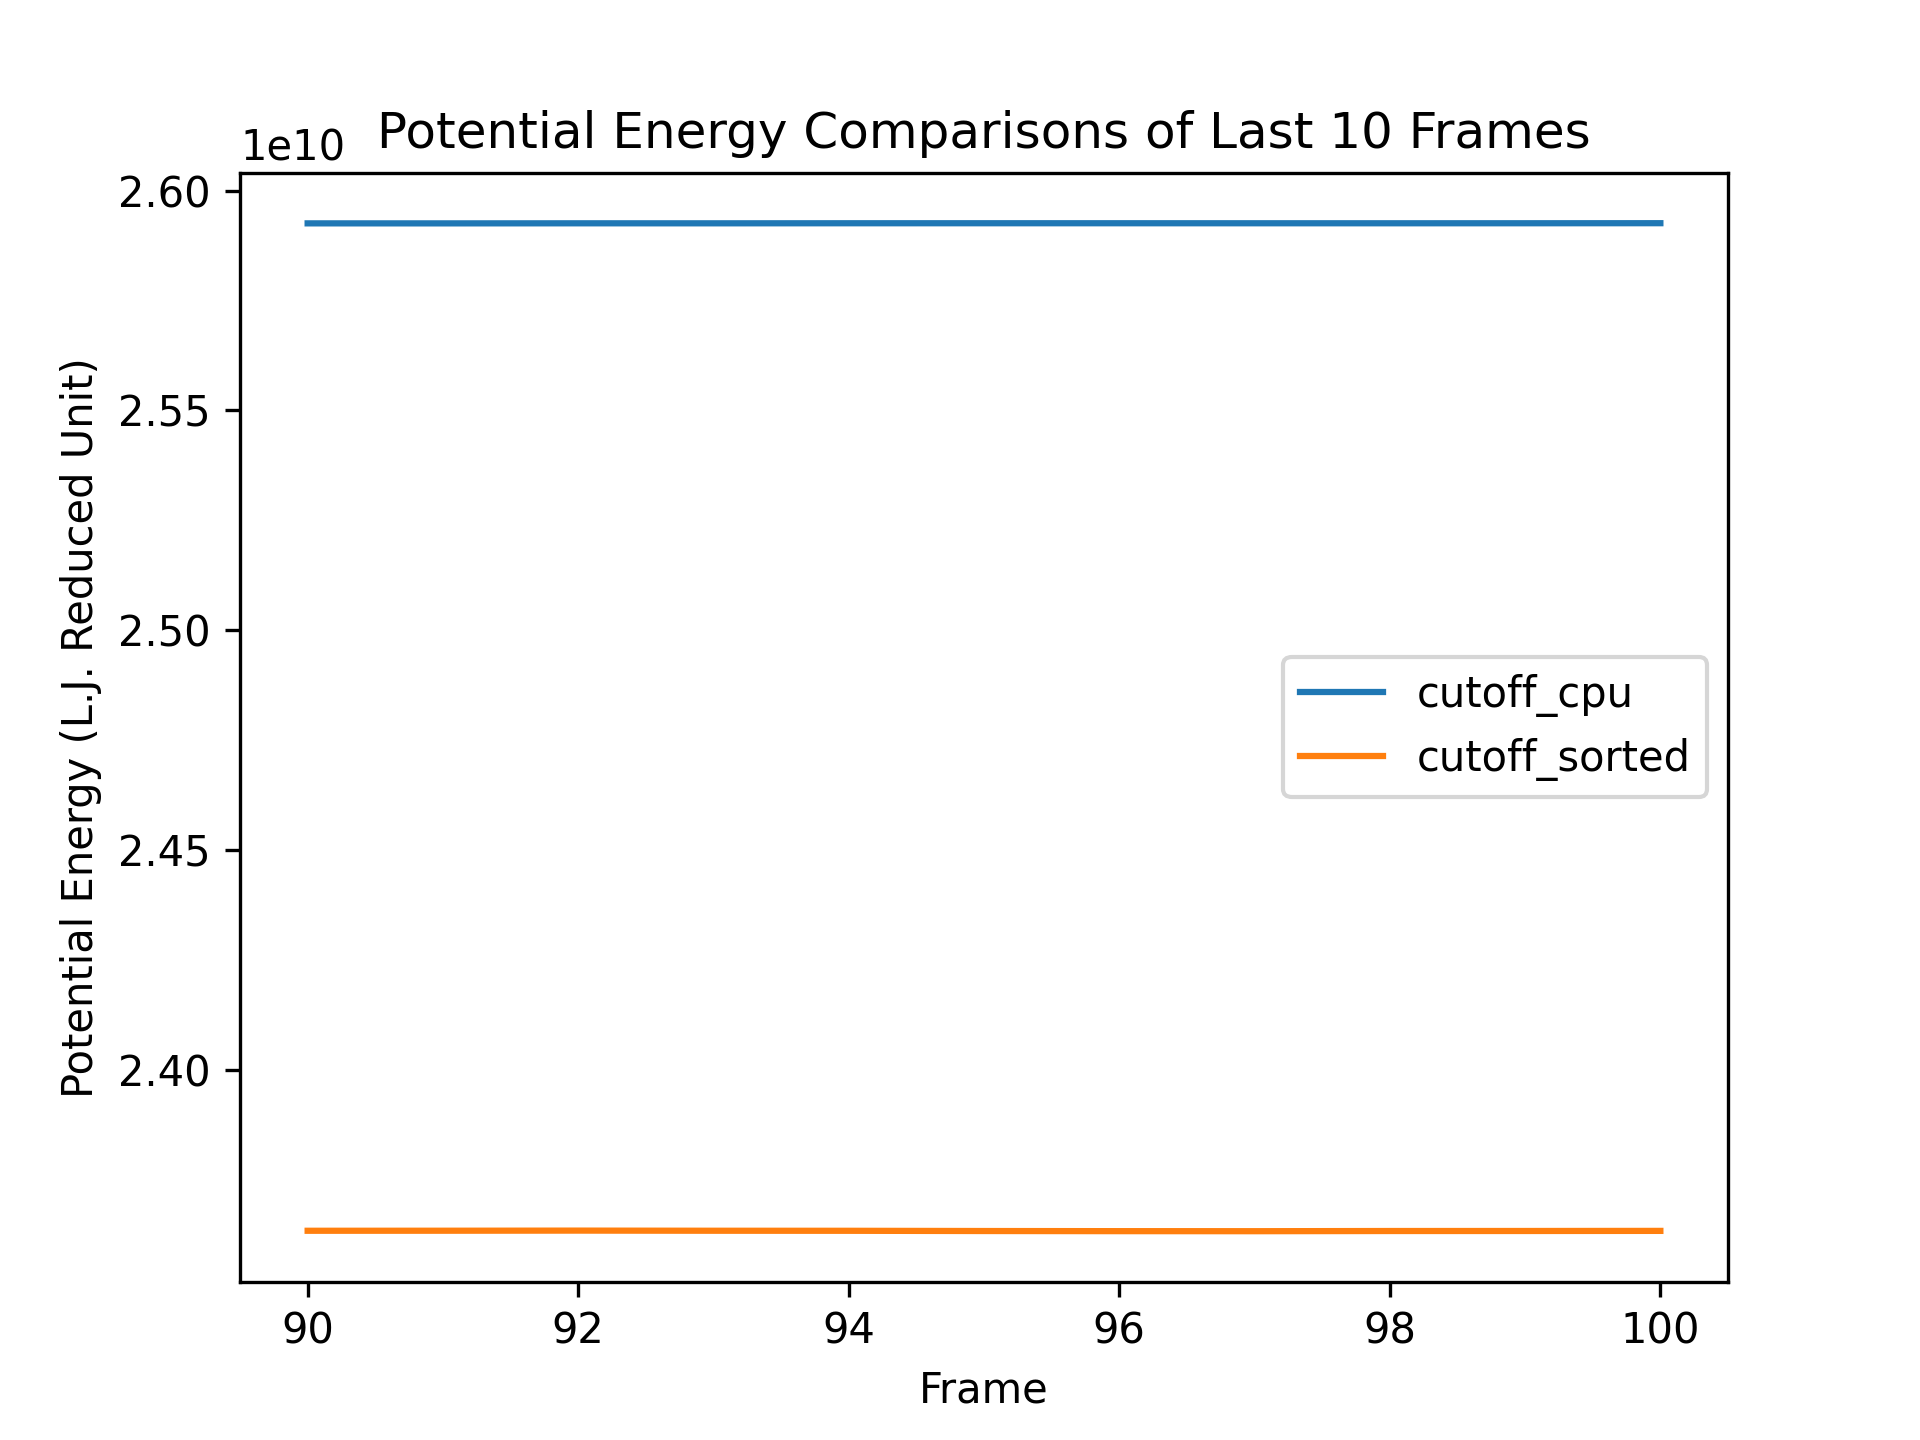
\includegraphics[width=\linewidth]{pe_cutoff.png}
        \caption{Cutoff Kernel Comparisons with Long-Range Corrections}
    \end{subfigure}

    \caption{Potential Energy Comparisons in the Last 10 Frames of a 1000-step integration between Different Exact and Cutoff Algorithms}
    \label{fig:pe_comp}
\end{figure}

\begin{figure}[h]
    \centering
    
    \begin{subfigure}{0.45\textwidth}
        \centering
        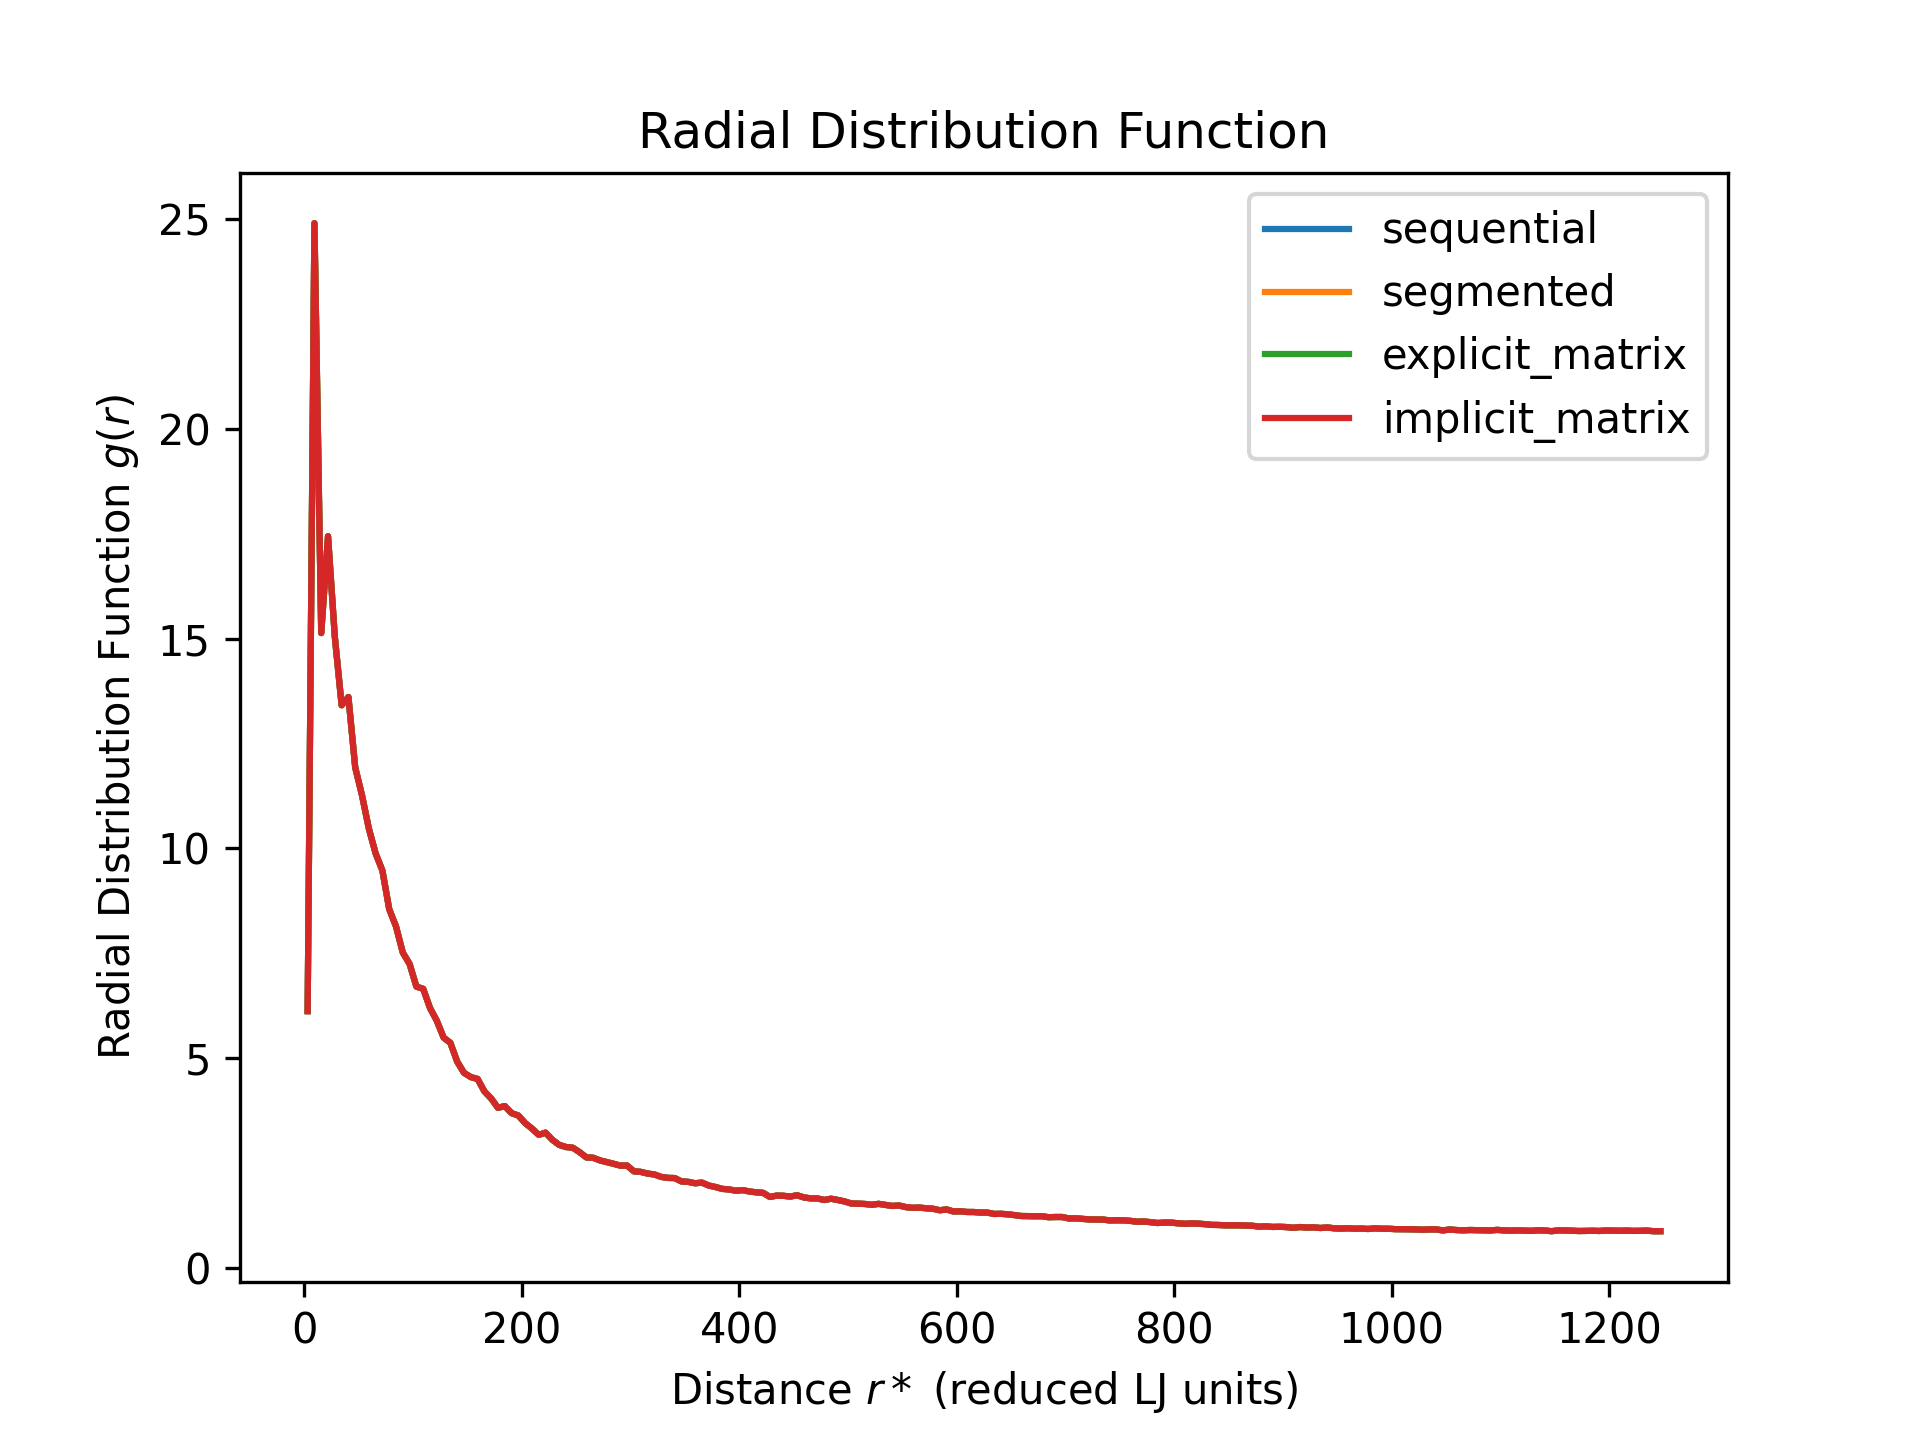
\includegraphics[width=\linewidth]{rdf_exact.png}
        \caption{Exact Kernel Comparisons}
    \end{subfigure}
    \hfill
    \begin{subfigure}{0.45\textwidth}
        \centering
        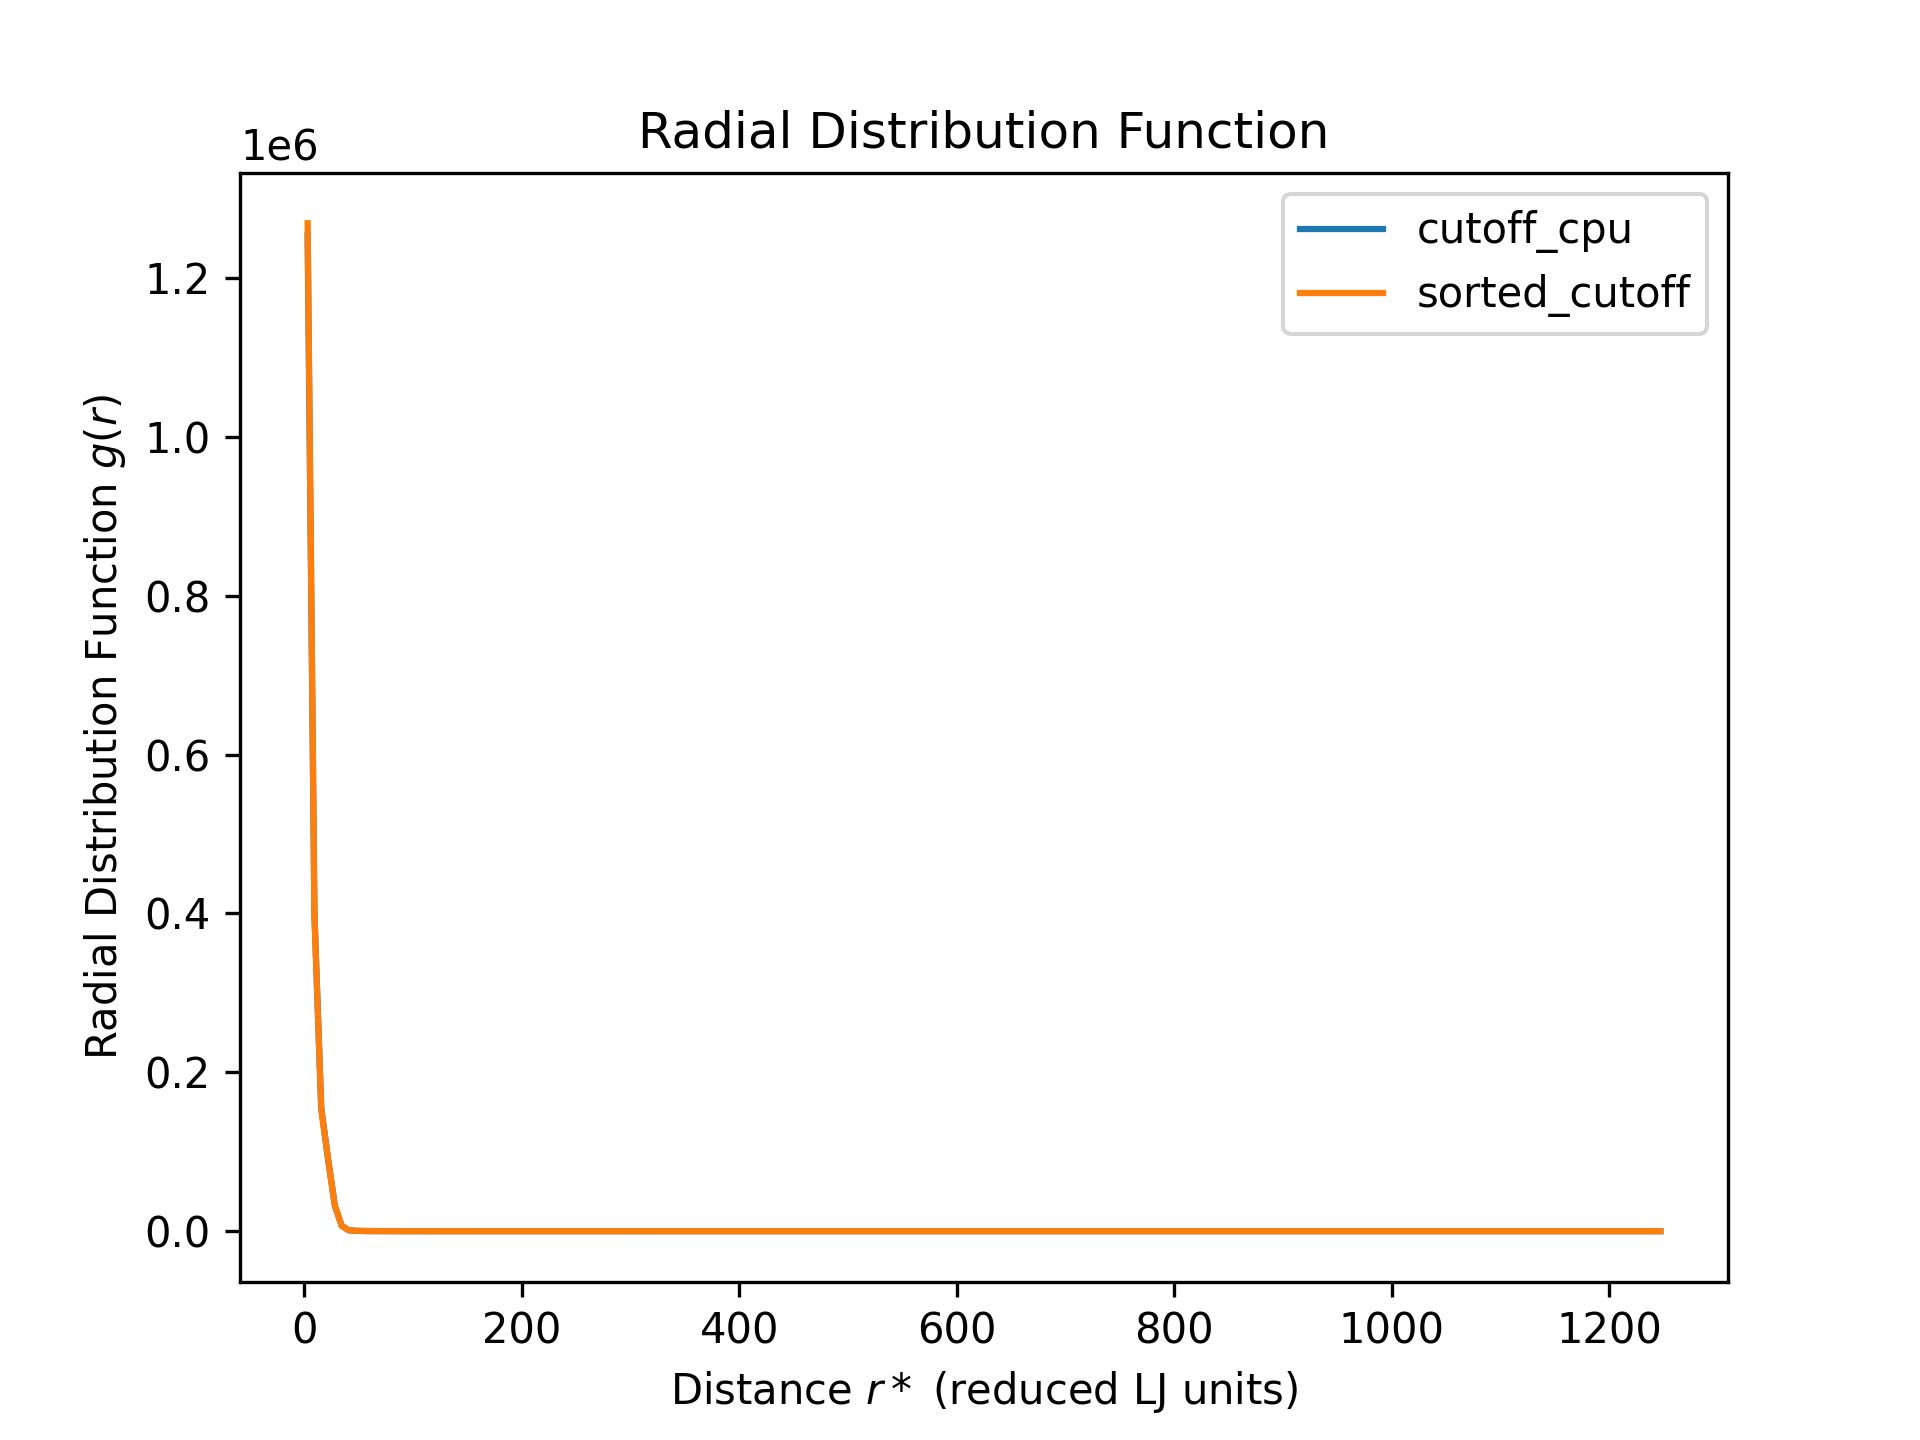
\includegraphics[width=\linewidth]{rdf_cutoff.png}
        \caption{Cutoff Kernel Comparisons}
    \end{subfigure}

    \caption{Comparisons of the average RDF in the Last 10 Frames of a 1000-step integration between Different Exact and Cutoff Algorithms}
    \label{fig:rdf_comp}
\end{figure}

\subsection{Runtime Experiments}

Comparing figures \ref{fig:forcePerformance} and \ref{fig:integrationPerformance}, we see that the performances of the entire MD simulation follow the same trend as the performances of the single force kernels, which confirms the force computation step as the bottleneck in an MD simulation. Both CPU algorithms have a quadratic run time with respect to $N$ (slope around 2 on the log-log plot), with the cutoff algorithm achieving a slight speedup compared with the exact algorithm, demonstrating the cost of pairwise force computations. Both force matrix methods achieve a quadratic empirical run time with a significant speedup (30x - 100x) compared to the sequential algorithm. The segmented traversal kernel starts off with a linear run time but grows to quadratic when $N$ gets closer to 10,000. Both cutoff kernels achieve a near constant run time. In fact, the run time of the cutoff kernels is largest when $N$ is at 1000 and slightly decreases with larger $N$.

\subsection{Hardware Experiments}
For the 1,000-atom case, the all-pairs force kernels show much higher SM utilization than the cutoff kernels. Both \texttt{calc\_force\_matrix} and \texttt{calc\_force\_matrix\_explicit} reach more than 80\% SM throughput, which suggests that these kernels are mainly compute-bound. In contrast, the cutoff kernels both \texttt{sorted} and \texttt{unsorted} have very low SM and memory throughput. This is mainly because the grid size is only 8 blocks, so there is not enough parallel work to fully occupy the GPU.

The \texttt{force\_mat\_sum} kernel behaves differently from the force computation kernels. It has lower SM throughput but much higher memory throughput, which indicates that this reduction stage is more limited by memory access than computation. The \texttt{atom\_label\_kernel} is very short, but it also suffers from low occupancy because the 1,000-atom problem size is too small.

For the 10,000-atom case, the cutoff kernels become much more efficient. Both \texttt{calc\_force\_cutoff\_gpu\_sorted} and \texttt{calc\_force\_cutoff\_gpu\_unsorted} reach around 78--79\% SM throughput, and their runtime is only tens of microseconds. This shows that the cutoff method scales much better when the number of atoms increases. The sorted cutoff version is slightly faster than the unsorted version in this experiment.

The all-pairs matrix kernels still have high SM throughput for 10,000 atoms, but their runtime becomes much larger because the amount of work grows quadratically with the number of atoms. The \texttt{force\_mat\_sum} kernel becomes strongly memory-bandwidth dominated, reaching 89.13\% memory throughput but only 11.34\% SM throughput. This suggests that the reduction stage is mainly limited by global memory traffic rather than arithmetic computation.

\section{Discussion}
% Analyze the results and their implications.
Between the three exact kernels, segmented traversal has the worst run time. Interestingly, it is also the only one that scales linearly when $N$ is small ($N\le3000$). Since each thread in its kernel has a span of $N$, when the total number of threads is small and fully parallelizable, it is expected that the run time of segmented traversal is $O(N)$. However, at $N=1000$, it only achieves a 10x speedup. Given that the sequential algorithm performs $\frac{999\times 1000}{2}$ computations, a speedup of 500x would have been expected. This gap could be explained by GPU under-utilization and memory access latencies, as well as kernel launch overheads. Even with a small block size of 32, only 32 blocks are launched in the grid, which leaves a large portion of the GPU idle. With this small block size, shared memory loading must be performed frequently, and global memory access is only reduced by a factor of 32, which becomes a bottleneck for the kernel. The sequential code, on the other hand, utilizes the CPU cache perfectly, which leads to higher compute throughput.

Although the force matrix methods scale quadratically with $N$, they perform much better at smaller $N$. This can be explained by their high compute throughput as seen in table \ref{tab:ncu_kernel_summary}. In the explicit method, each thread computes one entry in the force matrix, which maximally utilizes the parallel cores in the GPU. In the implicit method, each thread loops through the tile, which is coarsened compared to the explicit method but still leads to much higher GPU utilization than the segmented traversal kernel. In fact, the most significant advantage of the force matrix kernels is their high occupancies at smaller $N$. The explicit method launches $\frac{N(N-1)}{2}$ threads, each performing one computation; the implicit method launches $t\times \frac{(1+\frac{N}{t})\frac{N}{t}}{2}=\frac{N(1+\frac{N}{t})}{2}$ threads, each performing $t$ computations, where $t$ is the tile dimension.

At larger $N$, both methods get serialized on the GPU. The total computational work performed by the segmented traversal kernel is $N^2$. The explicit force matrix kernel performs $\frac{N(N-1)}{2}=O(N^2)$ work during the filling stage and $O(N)$ work during the reduction stage (note that summation during the reduction stage is much cheaper than force computations during the filling stage). The implicit force matrix kernel performs $t\times \frac{N(1+\frac{N}{t})}{2}=\frac{N(t+N)}{2}=O(N^2)$ work. Since all three methods perform $O(N^2)$ work, they have the same asymptotic time complexity when blocks are serialized on the GPU.

Although the implicit force matrix performs more actual force computations than the explicit method, it achieves the shortest run time at $N=10000$. As seen in table \ref{tab:ncu_kernel_summary_10000}, both kernels are compute bound. Therefore, this speedup cannot be explained by the use of shared memory in the implicit method. However, a key advantage of the coarsened approach of the implicit method is the amortization of heavy index calculations. Recall that mapping the 1-dimensional index of the collapsed storage array to row and column indices of the force matrix involves floating point operations and square roots, which leads to a large setup overhead. In the explicit method, each thread performs this calculation, but in the implicit method, only one thread in a block does. This means that the implicit method is wasting less computation resources on index calculations. Surprisingly, contention in global memory does not seem to slow down the implicit method. Even with privatization, it is expected that a maximum of $\frac{N}{t}$ threads can add to the same position in the global forces array simultaneously. It seems that the scheduling of the blocks may have prevented simultaneous accumulations to the same position. 

The parallel reduction stage of the explicit method is heavily memory bound with large $N$, which is expected given the random access patterns in the collapsed storage array that prevent memory coalescing. 

For the \texttt{Label/Cutoff Method}, both the runtime results and the hardware profiling results show that this method is strongly affected by the number of atoms. This is mainly because the kernel launch size is directly related to the number of atoms. When the system contains only a small number of atoms, only a small number of thread blocks are launched, so the GPU cannot be fully occupied. As a result, the SM throughput is low and the overhead of launching kernels becomes more noticeable. However, when the number of atoms increases, the cutoff method provides enough parallel work for the GPU. Therefore, both the SM throughput and the runtime performance improve significantly. One possible future optimization is to tune the block size. Using smaller blocks may increase the number of launched blocks and improve SM occupancy for smaller problem sizes.

For the comparison between the sorted and unsorted versions, our hypothesis is also supported by the results. Although a single round of force computation kernel may be slower in the sorted version because of the additional global memory access and index mapping, the overall simulation runtime is better than the unsorted version. This is because the sorted version avoids repeatedly recovering the atom positions back to the original order and allows the global position array to remain in a more cache- and memory-friendly layout. Therefore, the benefit is not only from the force kernel itself, but also from reducing repeated data movement across the full simulation loop. As the number of atoms becomes larger, we expect this advantage to become more significant because the cost of unnecessary global memory movement grows with the system size.

These results show that GPU performance depends on both algorithmic complexity and hardware utilization. Although the cutoff method reduces the number of pairwise interactions, it is not always efficient for small systems because the GPU does not receive enough parallel work. As the atom count increases, the cutoff method becomes much more effective because it both reduces unnecessary computation and provides enough work to better utilize the SMs. The comparison between the sorted and unsorted versions also shows the importance of data layout. Keeping atoms in sorted order can improve the total simulation runtime by reducing repeated memory movement, even if an individual kernel does not always appear faster. Therefore, an efficient GPU implementation should consider not only the mathematical algorithm, but also kernel launch size, occupancy, memory access pattern, and data movement across the full simulation loop.

\section{Conclusion}
% Provide final thoughts and potential future work.
In this paper, we implemented and analyzed different strategies to accelerate force computations in an MD simulation on the GPU. We reduced computations by half with the explicit force matrix, and further optimized memory usage using the implicit force matrix. Compared to the sequential algorithm, we achieved 30x to 100x speedup in a realistic problem size of $N\in [1000,10000]$. Noticing that the Lennard-Jones forces decay drastically at far distances, we implemented kernels with a cutoff distance that achieve constant run times, with speedup up to 1000x for $N=10000$ compared to the sequential algorithm. Although the exact methods yield identical ensemble properties of the simulation system, the cutoff methods deviate significantly from the expected behavior, which reveals physical flaws in the approach. Finally, we analyzed the kernel profiles and determined algorithmic bottlenecks.

Future work should be directed to identifying the flaw with the cutoff method. Although a cutoff of $2.5\sigma$ is conventional in MD simulations, it may be insufficient in our sparse system which lacks solvent to mediate interactions. In addition, it is possible that overstretching of the covalent bonds lead to incorrect omission of the bonded interactions.

In addition, we only implemented kernels for the linear monopolymer. Future study on adapting those kernels to heterogeneous systems and non-linear systems will help generalize the approach. In addition, solvent systems typically contain a much larger number of atoms and would benefit significantly from GPU acceleration.

Finally, simulation of an MD system is only the first step in an MD study. Much work remains on the analysis of the trajectories, which involves a large number of parallelizable operations, including pairwise energy calculations, trajectory alignment, and unwrapping of molecules in the unit cell. Future work could develop GPU kernels that accelerate the analysis of thousands of frames of trajectories.

\begin{thebibliography}{9}

\bibitem{cupy_argsort}
CuPy,
\textit{cupy.argsort Documentation}.
Available: \url{https://docs.cupy.dev/en/stable/reference/generated/cupy.argsort.html}.
Accessed: Apr. 26, 2026.

\end{thebibliography}

\end{document}
